% !TeX program = xelatex
% !TeX encoding = UTF-8 Unicode
\documentclass[UTF8,openany,12pt]{ctexbook}

\usepackage[a4paper]{geometry}
\usepackage{graphicx}
\usepackage{booktabs}
\usepackage{longtable}
\usepackage{array}
\usepackage{tabularx}
\usepackage{amsmath,amssymb}
\usepackage{float}
\usepackage{caption}
\usepackage{enumitem}
\usepackage{tocloft}
\usepackage{hyperref}
\usepackage{setspace}
\usepackage{xcolor}
\usepackage{tikz}
\usepackage[numbers,sort&compress]{natbib}
\usetikzlibrary{arrows.meta,positioning}

\geometry{
    top=2.54cm,
    bottom=2.54cm,
    left=3.17cm,
    right=3.17cm,
    headheight=1.2cm,
    headsep=0.4cm,
    footskip=1.6cm
}

\graphicspath{{../img/}}
\hypersetup{hidelinks}
\setlength{\parindent}{2em}
\setlength{\parskip}{0pt}
\linespread{1.35}
\raggedbottom

\DeclareCaptionFont{fsuwuhao}{\zihao{5}\songti}
\captionsetup{font=fsuwuhao,labelfont=normalfont,labelsep=space}
\captionsetup[figure]{justification=centering}
\captionsetup[table]{justification=centering,singlelinecheck=false,skip=6pt}

\setlength{\tabcolsep}{4.5pt}
\renewcommand{\arraystretch}{1.20}
\setcounter{secnumdepth}{3}
\setcounter{tocdepth}{2}
\pagestyle{plain}

\ctexset{
    chapter = {
        number = \arabic{chapter},
        format = \centering\heiti\zihao{-2},
        beforeskip = 24pt,
        afterskip = 18pt
    },
    section = {
        format = \raggedright\heiti\zihao{3},
        beforeskip = 18pt,
        afterskip = 6pt
    },
    subsection = {
        format = \raggedright\heiti\zihao{4},
        beforeskip = 12pt,
        afterskip = 6pt
    }
}

\newcommand{\keywords}[1]{\par\noindent{\heiti 关键词：}#1}
\newcommand{\engkeywords}[1]{\par\noindent{\bfseries Key words:}#1}
\newcommand{\formalmetric}[1]{\texttt{#1}}

\title{面向地下排水管道缺陷筛查的高召回门控选模与有效信息重加权研究}
\author{}
\date{2026年4月}

\begin{document}
\zihao{-4}\songti

\frontmatter

\chapter*{摘要}
\addcontentsline{toc}{chapter}{摘要}
地下排水管道缺陷识别在工程部署中同时面临三类约束：正常帧远多于缺陷帧，小样本与细粒度异常容易被背景纹理淹没，以及默认阈值下的分类指标并不能直接反映系统在高召回筛查中的减负收益。针对这一问题，本文将研究范围严格限定在 stage-1，并将第一阶段重新定义为 recall-constrained 的 Normal/Abnormal gate，而不是默认阈值二分类任务。本文的目标不是提出新的 detector，而是在已完成证据的基础上建立一套可复现、可审计的 stage-1 正式选模与增强协议。

在统一的 formal protocol 下，本文首先完成了两套容量扫描：其一是 direct binary gate 的 five-model capacity scan，其二是 source-side six-class capacity scan。前者使用 \formalmetric{Spec@R99.5}、\formalmetric{Spec@R99.0}、\formalmetric{Prec@R99.0} 与 \formalmetric{PTR@R99.0} 作为正式排序准则，并对每个 epoch checkpoint 执行温度校准与 operating-point 评估；后者仅作为 source-side representation 的辅助参考，按 Accuracy、AUROC 与 AUPRC 排序。实验结果表明，在 direct binary gate 的正式视图下，\texttt{yolo11m-cls} 取得最优综合表现，\texttt{yolo11x-cls} 为第二对照模型，而 \texttt{yolo11l-cls} 退居第三。与此同时，source six-class 视图得到的排序为 \texttt{x > m > l > s > n}，与 binary gate 视图的 \texttt{m > x > l > s > n} 并不一致。

在此基础上，本文进一步完成了以 \texttt{yolo11m-cls} 为主模型的 formal HN ratio sweep，以及以 \texttt{yolo11x-cls} 为第二模型的 light cross-capacity validation。结果表明，HN 的收益不是单调增加的；在当前正式排序规则下，\texttt{yolo11m-cls + hn14} 取得整条 sweep 的最优结果，其 \formalmetric{Spec@R99.5} 相比 \texttt{hn00} 提升 0.0476，而 \texttt{yolo11x-cls} 上的 \texttt{hn02} 则未能复现相同方向的净增益。该结果说明 HN 是建立在既有 capacity mainline 之上的模型相关增强，而不是对 backbone 选择的重新裁决。

此外，五个 binary gate 模型全部表现出 trainer \formalmetric{top1-best} 与 formal gate-best 的错位，说明 \formalmetric{top1} 虽然仍可作为训练健康信号，但并不对应高召回门控真正关心的 operating-point 目标，因而不应再被用作 stage-1 的正式 early-stop 或 checkpoint-selection 依据。在此基础上，本文进一步把 hard-normal pool 内部的样本价值异质性形式化为固定预算下的样本重分配问题，给出基于校准风险、一致性稳定性和结构支撑度的 Gate-Aligned Effective Information Score lite 框架，为后续训练侧增强提供统一的 stage-1 方法基础。综上，本文建立了围绕 formal gate-aware 选模、HN sweet spot 分析与样本效用重加权的 stage-1 证据链。
\keywords{地下排水管道；高召回门控；容量扫描；Hard-Negative 回流；样本效用重加权；温度校准；检查点选模；CCTV 图像}

\chapter*{Abstract}
\addcontentsline{toc}{chapter}{Abstract}
This manuscript focuses on stage-1 model selection and enhancement for sewer-defect screening under a high-recall operating regime. Rather than treating stage-1 as a default-threshold binary classifier, the study formalizes it as a recall-constrained Normal/Abnormal gate whose primary objective is normal filtering under fixed recall anchors. The contribution of the present work is therefore not a new detector, but a reproducible and auditable stage-1 protocol built on completed formal capacity scans and a completed hard-negative (HN) enhancement sweep.

Two formal capacity scans are first reported. The primary view is a direct binary-gate scan over five YOLO11 classification backbones, ranked by \formalmetric{Spec@R99.5}, \formalmetric{Spec@R99.0}, \formalmetric{Prec@R99.0}, and \formalmetric{PTR@R99.0}, with temperature scaling and operating-point evaluation applied to every epoch checkpoint. The auxiliary view is a six-class source-side scan ranked by Accuracy, AUROC, and AUPRC. The results show that \texttt{yolo11m-cls} is the formal leader under the binary gate objective, followed by \texttt{yolo11x-cls}, whereas the auxiliary six-class view ranks the models as \texttt{x > m > l > s > n}. This mismatch indicates that source-side representation quality cannot replace gate-aware checkpoint selection for stage-1.

The study then reports a formal HN ratio sweep on the selected main model \texttt{yolo11m-cls}, together with a light cross-capacity validation on \texttt{yolo11x-cls}. The HN gains are non-monotonic rather than monotonic. Under the same gate-aware ranking rule, \texttt{yolo11m-cls + hn14} becomes the formal HN winner, improving \formalmetric{Spec@R99.5} by 0.0476 over the \texttt{hn00} anchor, whereas \texttt{yolo11x-cls + hn02} does not reproduce the same directional gain. This evidence suggests that HN should be interpreted as a model-dependent stage-1 enhancement rather than a backbone-independent effect.

The experiments further show that trainer-selected \formalmetric{top1-best} checkpoints do not align with gate-selected checkpoints for any of the five binary-gate models. Trainer-side \formalmetric{top1} therefore remains useful for optimization-health monitoring, but should not be used as the official early-stopping or model-selection criterion for a high-recall gate. Building on these completed stage-1 findings, the thesis further formulates a Gate-Aligned Effective Information Score lite framework for fixed-budget hard-negative reweighting, so that replay probabilities can be redistributed within the existing top250 hard-normal pool without changing the total HN14 budget. The present thesis is therefore organized as a stage-1 mainline study centered on formal gate-aware model selection, HN sweet-spot analysis, and sample-utility-driven reweighting.
\engkeywords{sewer inspection, high-recall gate, capacity scan, hard-negative mining, sample valuation, temperature scaling, checkpoint selection, CCTV imagery}

\tableofcontents
\listoffigures
\listoftables

\chapter*{主要符号与缩略语说明}
\addcontentsline{toc}{chapter}{主要符号与缩略语说明}
\begin{longtable}{p{3.2cm}p{10.4cm}}
\toprule
符号/缩略语 & 含义 \\
\midrule
\endfirsthead
\toprule
符号/缩略语 & 含义 \\
\midrule
\endhead
\formalmetric{Spec@R99.5} & 在召回率不低于 99.5\% 的约束下，正常样本拦截能力所对应的 specificity。 \\
\formalmetric{Spec@R99.0} & 在召回率不低于 99.0\% 的约束下，正常样本拦截能力所对应的 specificity。 \\
\formalmetric{Prec@R99.0} & 在召回率不低于 99.0\% 的约束下的 precision。 \\
\formalmetric{PTR@R99.0} & 在召回率不低于 99.0\% 时的 pass-through rate，即进入下一阶段的样本占全部样本的比例。 \\
val-cal / val-op & 温度校准子集与 operating-point 评估子集。 \\
HN & Hard-Negative，指从训练 normal 中构造的高风险回流样本。 \\
GAEIS & Gate-Aligned Effective Information Score，本文用于固定预算样本效用重加权的评分框架。 \\
$\tau_{99.5}, \tau_{99.0}$ & 在 formal gate 评估下分别对应 \formalmetric{R99.5} 与 \formalmetric{R99.0} 的 operating threshold。 \\
\bottomrule
\end{longtable}

\mainmatter

\chapter{绪论}

\section{研究背景与工程意义}
地下排水管网是城市基础设施体系中的关键组成部分，其运行状态直接关系到城市防涝、道路安全以及水环境治理 \cite{moradi2019review,haurum2020survey,ma2026stateoftheart}。当前工程实践仍主要依赖 CCTV 巡检与人工复核，但海量正常帧、复杂背景纹理以及跨设备成像差异，使人工判读在效率、一致性和误报控制方面面临明显瓶颈 \cite{haurum2020survey,cheng2018deep}。因此，如何在保持缺陷高召回的前提下尽可能减少进入后续人工复核或后级检测的正常样本，已经成为 sewer inspection 智能化中的核心问题之一。

传统研究通常把第一阶段视作普通分类任务，默认以 Accuracy 或 \formalmetric{top1} 作为早停和选模依据。然而，在实际两阶段工作流中，stage-1 的职责并不是在默认阈值下取得最高整体分类分数，而是在固定高召回约束下最大化正常样本拦截。因此，默认阈值分类语义与高召回门控语义之间存在明显错位。本文据此将 stage-1 明确重定义为 recall-constrained gate，并围绕这一目标重新组织容量扫描、校准评估、checkpoint 选择以及 HN 增强分析。

\section{国内外研究现状}
\subsection{排水管道缺陷视觉识别}
排水管道缺陷识别经历了由人工特征到深度视觉模型的技术演进。早期工作以 HOG、SVM 和规则驱动候选区域为主，已经证明 CCTV 图像中的管道异常具有一定可计算性，但方法对场景变化较为敏感 \cite{halfawy2014hogsvm}。随着深度学习的发展，研究开始转向图像级分类与目标检测。Kumar 等利用深度卷积网络完成 sewer CCTV 缺陷分类，Cheng 等进一步将深度模型用于管道缺陷检测，表明数据驱动表征能够显著提升识别性能 \cite{kumar2018cnn,cheng2018deep}。

\subsection{YOLO 路线与 sewer 场景适配}
YOLO 系列因具备较好的实时性和工程成熟度，已成为管道缺陷检测中的常见基础路线 \cite{redmon2016yolo}。在 sewer 场景中，研究者围绕特征增强、轻量化部署与场景适配提出了多种改进策略，例如改进 YOLOv5 的管道缺陷检测模型以及轻量化 YOLOv5-Sewer 等 \cite{wang2023improvedyolov5,zhao2024yolov5sewer}。这些工作证明，YOLO 路线具有良好的工程基础；但它们也表明，不同任务目标之间不能简单共享同一评价口径：用于目标检测的 detector 精度并不直接回答高召回门控下的 normal filtering 问题。

\subsection{高召回分类、概率校准与约束优化研究}
Sewer-ML 数据集的发布为 sewer defect classification 提供了统一的 benchmark 条件，也使多尺度容量比较与 source-side representation 分析成为可能 \cite{haurum2021sewerml}。另一方面，温度校准已被证明是改善神经网络输出分数可信度的低成本方式，在不改变样本排序的前提下，有助于建立更稳定的 operating-point 比较基础 \cite{guo2017calibration}。此外，迁移学习在线路缺陷检测中的应用也已显示出缓解目标域标注不足的价值 \cite{situ2023transfer}。然而，就本文当前已完成证据而言，最需要优先解决的问题并不是 detector 结构本身，而是 stage-1 的正式任务边界、正式选模规则以及在正式主线固定后的训练侧增强方式。

\subsection{难样本挖掘、数据剪枝与样本效用建模研究}
围绕样本选择与训练效率提升，已有研究从 hard negative mining、uncertainty-driven selection、diversity-aware active learning、training-dynamics pruning 以及结构支撑建模等多个方向展开。相关工作共同指出，样本价值并不等于单一损失大小或原始不确定性，高风险样本中同样可能混入不稳定噪声与孤立异常点；因此，样本选择需要同时考虑风险、稳定性与结构支撑等因素 \cite{koh2017influence,ash2020badge,wu2022entropy,yang2024plug,kim2024structural,zhang2024tdds}。这一线索直接支撑了本文从 uniform HN replay 进一步走向固定预算样本重加权的研究动机。

\begin{table}[H]
    \centering
    \caption{相关研究分类与本文切入点}
    \label{tab:related-work-map}
    \begin{tabularx}{\textwidth}{p{3.1cm}p{3.1cm}Xp{2.3cm}}
        \toprule
        研究方向 & 代表任务对象 & 典型回答的问题 & 与本文关系 \\
        \midrule
        sewer / pipe defect 视觉识别 & CCTV 图像分类或检测 & 管道缺陷能否被机器视觉识别 & 提供场景背景与 benchmark 语境 \\
        YOLO / detector 场景适配 & detector 结构与部署效率 & 如何提升定位精度或实时性 & 仅提供工程背景，不直接回答 stage-1 gate 选模 \\
        calibration / constrained optimization & 概率分数与 operating point & 固定召回下如何稳定比较模型 & 直接支撑 formal gate-aware 协议 \\
        hard negative / sample valuation & 样本选择与训练效率 & 哪些样本更值得被重复学习 & 直接支撑 HN 与 fixed-budget reweighting \\
        \bottomrule
    \end{tabularx}
\end{table}

\begin{table}[H]
    \centering
    \caption{本文与已有工作的差异定位}
    \label{tab:thesis-difference-positioning}
    \begin{tabularx}{\textwidth}{p{3.1cm}XX}
        \toprule
        比较维度 & 常见 detector / classification 工作 & 本文定位 \\
        \midrule
        任务边界 & 直接优化 detector 或默认阈值分类精度 & 严格限定在 stage-1 recall-constrained gate \\
        正式主目标 & mAP、Accuracy、trainer-side \formalmetric{top1} & \formalmetric{Spec@R99.5 > Spec@R99.0 > Prec@R99.0 > PTR@R99.0} \\
        主问题 & 如何提升整体系检测或分类性能 & 如何 formalize stage-1 选模、HN 与样本效用重加权 \\
        训练增强位置 & 往往与 backbone / loss / detector 结构耦合 & 在已固定 mainline 上比较 HN 与 fixed-budget replay \\
        完整度边界 & 常直接给 detector 或系统级结论 & 不对完整两阶段系统优劣作超证据结论 \\
        \bottomrule
    \end{tabularx}
\end{table}

\section{研究问题与研究目标}
\subsection{本文的任务边界}
本文的任务边界被严格限定在 stage-1 前端筛查，而不是完整两阶段系统。更具体地说，本文只讨论基于 YOLO11-cls 的 high-recall gate 如何在固定召回约束下完成 formal backbone 选模、checkpoint 选择与训练侧增强；对 detector 结构、系统级闭环收益以及单阶段与两阶段系统的最终优劣比较，本文均不作正式结论。这一边界既符合当前已完成实验的真实范围，也使整篇论文的论证能够围绕同一 formal objective 展开。

\subsection{核心科学问题与研究目标}
围绕当前任务边界，本文重点回答三类相互衔接的问题。第一，在统一的 stage-1 formal protocol 下，哪一种 YOLO11-cls 容量最适合作为高召回 gate 的正式主模型。第二，在主模型固定后，HN 回流能否在同一 formal evaluator 下形成可排序、可解释的净增益，以及该增益是否具有模型相关性。第三，在 fixed-budget 的 HN14 working set 中，uniform replay 是否忽略了池内样本价值异质性，从而为后续样本效用重加权提供研究空间。

据此，本文的研究目标可以概括为：一是建立可复现、可审计的 stage-1 formal 选模协议；二是完成 backbone 容量扫描、cross-view mismatch 与 HN sweet spot 的证据闭环；三是在此基础上提出面向固定预算的样本效用重加权框架，为后续 stage-1 训练侧优化提供统一方法接口。

\section{研究内容与技术路线}
本文的技术路线由四个递进阶段组成。首先，在 direct binary gate 与 source six-class 两个视图上分别执行 formal capacity scan，并通过 temperature scaling、threshold sweep 与外部 gate-aware evaluator 确定正式 backbone 排序。其次，以 binary gate 视图下的主模型 \texttt{yolo11m-cls} 为起点，执行完整 HN ratio sweep，并在 \texttt{yolo11x-cls} 上做 light cross-capacity validation，用以判断 HN 收益的 sweet spot 与模型相关性。再次，结合 HN 曲线的非单调性以及 hard-normal pool 的内部异质性，本文把“比例扫描”进一步抽象为“固定预算下的样本重分配”问题，并提出 Gate-Aligned Effective Information Score lite 作为后续重加权框架。最后，全文通过 manifest、summary、registry 和 appendix source-of-truth 保证结果可复现与可审计。

\begin{figure}[H]
    \centering
    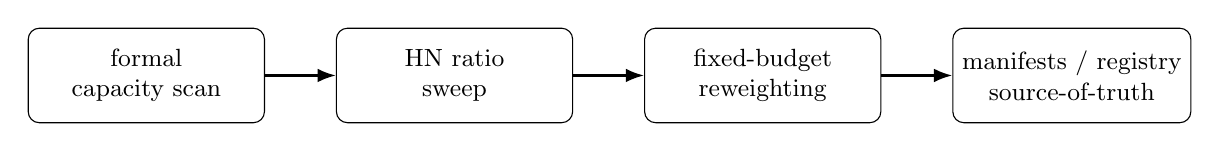
\begin{tikzpicture}[
        font=\small,
        box/.style={draw, rounded corners, align=center, minimum width=3.0cm, minimum height=1.2cm},
        arr/.style={-Latex, thick}
    ]
        \node[box] (a) {formal\\capacity scan};
        \node[box, right=0.9cm of a] (b) {HN ratio\\sweep};
        \node[box, right=0.9cm of b] (c) {fixed-budget\\reweighting};
        \node[box, right=0.9cm of c] (d) {manifests / registry\\source-of-truth};
        \draw[arr] (a) -- (b);
        \draw[arr] (b) -- (c);
        \draw[arr] (c) -- (d);
    \end{tikzpicture}
    \caption{本文的 stage-1 主线技术路线图}
    \label{fig:stage1-mainline-roadmap}
\end{figure}

\begin{figure}[H]
    \centering
    \begin{tikzpicture}[
        font=\small,
        box/.style={draw, rounded corners, align=center, minimum width=4.1cm, minimum height=1.3cm},
        note/.style={draw, dashed, align=center, minimum width=2.8cm, minimum height=1.0cm},
        arr/.style={-Latex, thick}
    ]
        \node[box] (s1) {Stage-1\\high-recall gate};
        \node[box, right=2.0cm of s1] (s2) {Stage-2\\detector / human review};
        \node[note, above=0.9cm of s1] (scope) {本文覆盖范围};
        \draw[arr] (s1) -- (s2);
        \draw[arr] (scope) -- (s1);
    \end{tikzpicture}
    \caption{当前研究问题在完整两阶段系统中的位置}
    \label{fig:stage1-in-system}
\end{figure}

\section{主要创新点}
围绕上述主线，本文的主要创新点体现在以下三个方面：
\begin{enumerate}[label=\arabic*.]
    \item 将 stage-1 重新界定为 recall-constrained high-recall gate，并给出一套由 temperature scaling、val-cal/val-op 划分、epoch-level evaluator 和 gate-aware checkpoint selection 共同构成的 formal 协议。
    \item 完成两套 formal capacity scan 与主模型上的 HN ratio sweep，给出从 backbone 选择、checkpoint 错位到 HN sweet spot 的系统性 stage-1 证据链，并明确 direct binary gate 才是正式主裁判视图。
    \item 在 HN 非单调收益和 hard-normal candidate pool 异质性的基础上，提出面向固定预算的 Gate-Aligned Effective Information Score lite 重加权框架，将训练侧增强问题从“回流比例”推进到“池内样本效用”层面。
\end{enumerate}

\section{论文组织结构}
全文围绕 stage-1 主线的 formal 选模、训练侧增强和样本重加权展开。第 2 章介绍高召回门控的理论基础、指标定义和样本效用建模动机；第 3 章说明数据集、实验平台和 formal working set 的组织方式；第 4 章集中报告 direct binary gate capacity scan、six-class source 辅助视图以及 cross-view rank mismatch；第 5 章报告主模型上的 HN ratio sweep 与 cross-capacity validation；第 6 章给出基于有效信息量的非线性样本重加权方法及 lite 消融设计；第 7 章总结当前已建立的 stage-1 证据链及其工程启示；附录部分进一步补充 formal protocol、HN provenance 以及信息量重加权的复现接口与 source-of-truth 清单。

\section{本章小结}
本章从工程需求、任务边界、研究问题与技术路线四个层面明确了本文的写作中心：当前工作不是 detector 结构论文，也不是系统级两阶段优劣比较论文，而是一篇围绕 stage-1 高召回门控 formal 化、HN 训练侧增强以及固定预算样本重加权展开的主线论文。后续章节的全部理论、图表和结论，均围绕这一主线组织。

\chapter{理论基础与关键技术}

\section{stage-1 高召回门控的目标定义}
设 stage-1 的输入样本总数为 $N$。其中 abnormal 样本需要尽可能完整地保留给后续人工复核或后级处理，而 normal 样本应在尽可能不牺牲召回的前提下被前级拦截。由此，stage-1 的核心目标并不是默认阈值下的总体分类正确率，而是高召回约束下的 normal filtering ability。

本文采用两个固定工作点作为正式锚点：\formalmetric{Recall$\geq$99.5\%} 与 \formalmetric{Recall$\geq$99.0\%}。在这两个约束下，正式排序规则定义为：
\begin{equation}
\formalmetric{Spec@R99.5} \succ \formalmetric{Spec@R99.0} \succ \formalmetric{Prec@R99.0} \succ \formalmetric{PTR@R99.0}.
\end{equation}

\section{正式指标定义}
在二分类 gate 语境中，\formalmetric{Spec@R99.5} 与 \formalmetric{Spec@R99.0} 分别表示在满足相应召回约束时的 specificity；\formalmetric{Prec@R99.0} 表示在 \formalmetric{Recall$\geq$99.0\%} 约束下的 precision。本文特别采用 \formalmetric{PTR@R99.0} 作为第四排序准则，其含义为在 \formalmetric{Recall$\geq$99.0\%} 对应阈值下的 pass-through rate，即仍被送往下一阶段的样本占全部样本的比例：
\begin{equation}
\formalmetric{PTR@R99.0} = \frac{TP + FP}{N}.
\end{equation}
为便于后续统一讨论，本文同时给出 recall、specificity 与 precision 的定义。记异常类样本总数为 $P$、正常类样本总数为 $N_{\mathrm{neg}}$，则
\begin{equation}
\mathrm{Recall} = \frac{TP}{TP + FN},
\end{equation}
\begin{equation}
\mathrm{Specificity} = \frac{TN}{TN + FP},
\end{equation}
\begin{equation}
\mathrm{Precision} = \frac{TP}{TP + FP}.
\end{equation}
其中，\formalmetric{Spec@R99.5} 与 \formalmetric{Spec@R99.0} 均是带有 operating-point 约束的条件量，而 \formalmetric{PTR@R99.0} 则直接刻画固定高召回条件下进入下一阶段的样本负担，因此既具有统计意义，也具有工程意义。

\begin{table}[H]
    \centering
    \caption{常用默认分类指标与本文 formal 指标的差异}
    \label{tab:formal-metric-difference}
    \begin{tabularx}{\textwidth}{p{3.2cm}XX}
        \toprule
        比较维度 & 默认阈值分类指标 & 本文 formal gate 指标 \\
        \midrule
        典型代表 & Accuracy、trainer-side \formalmetric{top1}、loss & \formalmetric{Spec@R99.5}、\formalmetric{Spec@R99.0}、\formalmetric{Prec@R99.0}、\formalmetric{PTR@R99.0} \\
        operating point & 通常隐含固定默认阈值 & 通过 val-cal 与 val-op 明确求取 \\
        关注对象 & 总体分类正确率或训练健康状态 & 固定高召回条件下的 normal filtering 能力 \\
        对 stage-1 的适配性 & 可监控训练，但不能直接拍板正式 winner & 直接决定 checkpoint selection 与 mainline 排序 \\
        \bottomrule
    \end{tabularx}
\end{table}

\section{温度校准与 gate-aware checkpoint selection}
为避免不同 checkpoint 的分数尺度不可比，本文对每个 epoch checkpoint 采用单标量 temperature scaling \cite{guo2017calibration}。具体流程如下：
\begin{enumerate}[label=\arabic*.]
    \item 在固定的 val-cal 子集上拟合温度参数 $T$；
    \item 将该温度应用于 val-op 子集，得到 calibrated score；
    \item 在 val-op 上执行 threshold sweep，计算候选阈值下的 recall、specificity、precision 与 pass-through rate；
    \item 按照正式排序规则选出 gate-best checkpoint，而不是直接使用 trainer 自动保存的 \texttt{best.pt}。
\end{enumerate}

这一协议意味着 calibration 已经内嵌为 formal evaluation 的组成部分，而不是独立于容量扫描之外的附加训练阶段。trainer-side 的 \formalmetric{acc/top1/loss} 仍然保留，但只承担训练健康监控功能，不承担正文正式选模功能。

\begin{figure}[H]
    \centering
    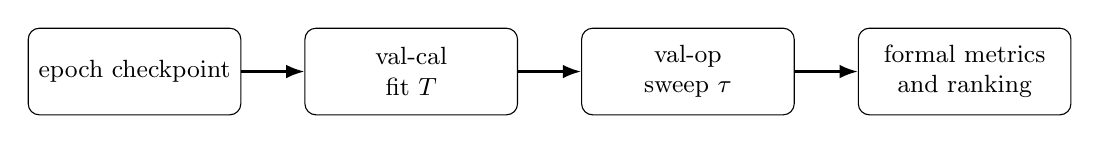
\begin{tikzpicture}[
        font=\small,
        box/.style={draw, rounded corners, align=center, minimum width=2.7cm, minimum height=1.1cm},
        arr/.style={-Latex, thick}
    ]
        \node[box] (ckpt) {epoch checkpoint};
        \node[box, right=0.8cm of ckpt] (cal) {val-cal\\fit $T$};
        \node[box, right=0.8cm of cal] (sweep) {val-op\\sweep $\tau$};
        \node[box, right=0.8cm of sweep] (rank) {formal metrics\\and ranking};
        \draw[arr] (ckpt) -- (cal);
        \draw[arr] (cal) -- (sweep);
        \draw[arr] (sweep) -- (rank);
    \end{tikzpicture}
    \caption{temperature scaling 与 threshold sweep 的 formal 工作流}
    \label{fig:calibration-threshold-flow}
\end{figure}

\section{高召回约束下的非对称学习问题}
从目标形式看，stage-1 不是一个“最大化总体准确率”的对称二分类问题，而是一个“在固定高召回条件下最大化正常样本拦截能力”的非对称学习问题。这一目标可写成如下 constrained form：
\begin{equation}
\max_{\theta,\tau}\ \mathrm{Specificity}(\theta,\tau)
\quad
\text{s.t.}\quad
\mathrm{Recall}(\theta,\tau)\ge R^\ast,
\end{equation}
其中 $\theta$ 表示模型参数，$\tau$ 表示 operating threshold，$R^\ast$ 为预先设定的召回下界。与默认阈值分类不同，这一目标本质上属于“固定一个 rate 再优化另一个 rate”的 rate-constrained learning \cite{kumar2021constrained}。因此，trainer 侧报告的 \formalmetric{top1} 或默认验证精度并不天然对应本文真正关心的 formal gate objective。

\begin{figure}[H]
    \centering
    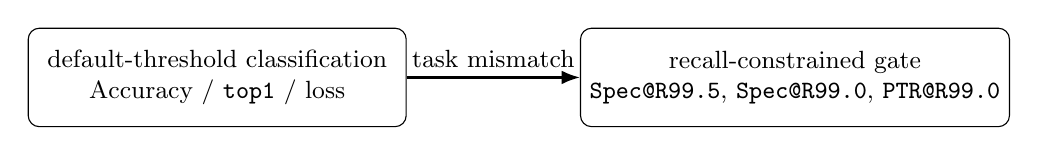
\begin{tikzpicture}[
        font=\small,
        box/.style={draw, rounded corners, align=center, minimum width=4.8cm, minimum height=1.25cm},
        arr/.style={-Latex, thick}
    ]
        \node[box] (left) {default-threshold classification\\Accuracy / \formalmetric{top1} / loss};
        \node[box, right=2.2cm of left] (right) {recall-constrained gate\\\formalmetric{Spec@R99.5}, \formalmetric{Spec@R99.0}, \formalmetric{PTR@R99.0}};
        \draw[arr] (left) -- node[above]{task mismatch} (right);
    \end{tikzpicture}
    \caption{默认阈值分类与 recall-constrained gate 的差异}
    \label{fig:default-vs-gate}
\end{figure}

\section{难样本挖掘与样本效用建模}
HN 回流的直接动机是：训练阶段存在一批被当前 gate 赋予较高 abnormal 风险的 normal 样本，重复学习这些样本可能提升固定高召回条件下的正常样本拦截能力。然而，uniform hard replay 隐含了一个更强的前提，即 hard pool 内部样本价值近似同质。当前 HN 曲线的非单调性表明，这一前提并不稳固；高风险样本并不等于高效样本，极端高分样本中可能同时混入 acquisition noise、模糊、反光或 feature-space 中的孤立异常点。

这一判断与样本影响分析、主动选择与结构化样本价值建模文献的结论一致。Koh 与 Liang 指出，训练样本的价值不应只由表面损失大小决定，还应考虑其对目标函数的实际影响 \cite{koh2017influence}。BADGE 及其后续工作表明，不确定性与多样性应被联合考虑，而不能只依赖单一 uncertainty proxy \cite{ash2020badge,wu2022entropy,yang2024plug}。Kim 等与 Zhang 等进一步强调了结构支撑和训练动态对样本价值判断的重要性 \cite{kim2024structural,zhang2024tdds}。因此，基于已完成的 capacity scan 与 HN 结果，把“比例扫描”进一步推进为“固定预算下的样本效用重加权”是自然且必要的下一步。

\begin{table}[H]
    \centering
    \caption{样本效用建模中三类关键信号的作用}
    \label{tab:sample-valuation-signals}
    \begin{tabularx}{\textwidth}{p{2.6cm}p{3.3cm}Xp{2.3cm}}
        \toprule
        信号类型 & 可观测量 & 作用机制 & 在本文中的对应 \\
        \midrule
        风险信号 & 校准后 abnormal score 与 threshold margin & 放大真正靠近 formal gate 边界的 normal & $R_i$ \\
        稳定性信号 & 轻量 TTA 下的 logit variance & 抑制高风险但极不稳定的伪难例 & $C_i$ \\
        结构支撑信号 & feature-space 邻域相似度 & 区分系统性困难模式与孤立异常点 & $D_i$ \\
        \bottomrule
    \end{tabularx}
\end{table}

\begin{figure}[H]
    \centering
    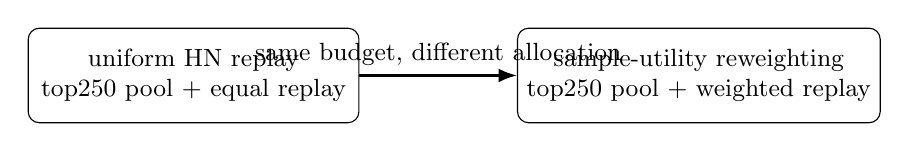
\begin{tikzpicture}[
        font=\small,
        box/.style={draw, rounded corners, align=center, minimum width=4.2cm, minimum height=1.2cm},
        arr/.style={-Latex, thick}
    ]
        \node[box] (u) {uniform HN replay\\top250 pool + equal replay};
        \node[box, right=2.0cm of u] (w) {sample-utility reweighting\\top250 pool + weighted replay};
        \draw[arr] (u) -- node[above]{same budget, different allocation} (w);
    \end{tikzpicture}
    \caption{uniform HN 与固定预算样本重加权的区别}
    \label{fig:uniform-vs-weighted}
\end{figure}

\section{six-class source 视图的辅助地位}
除 direct binary gate 外，本文还组织了一条 six-class source 容量扫描，用于观察不同容量模型在 source-side representation 任务上的相对位置。该视图的正式排序规则为 Accuracy、AUROC 与 AUPRC。然而，这一视图只承担辅助参考角色，不应替代 direct binary gate 的正式 backbone 选择。

\section{本章小结}
本章从任务定义、指标体系、温度校准、固定召回约束优化以及样本效用建模动机五个方面，为后续实验章节提供了统一理论基础。尤其是 PTR 的工程含义、trainer-side 指标与 formal objective 的错位来源，以及样本价值不应由单一 loss 或 raw uncertainty 决定的判断，共同构成了本文 stage-1 主线的理论支点。

\chapter{数据集构建、实验平台与 formal 工作流}

\section{数据来源与数据组织}
本文使用两套 source-side 数据集来支撑当前 stage-1 研究。第一套是 direct binary gate 数据集 \texttt{sewerml\_gate2\_train7200}，共 7200 张图像，其中训练集 6480 张、验证集 720 张；类别分布为 abnormal 6000 张、normal 1200 张。第二套是 six-class source 数据集 \texttt{sewerml\_cls6\_train7200}，同样包含 7200 张图像，并被均衡组织为六个类别，每类 1200 张，训练集与验证集分别为 6480 与 720 张。

对于 binary gate formal protocol，全部 720 张验证图像进一步按类别分层拆分为 val-cal 与 val-op 两部分，其中 val-cal 为 216 张，val-op 为 504 张；对应 abnormal/normal 的划分分别为 180/36 与 420/84。该拆分仅用于温度参数拟合与 operating-point 报告，不参与训练。

\begin{table}[H]
    \centering
    \caption{stage-1 数据集统计}
    \label{tab:stage1-dataset-stats}
    \begin{tabular}{lcccc}
        \toprule
        Dataset & Total & Train & Val & Class Distribution \\
        \midrule
        \texttt{sewerml\_gate2\_train7200} & 7200 & 6480 & 720 & abnormal 6000 / normal 1200 \\
        \texttt{sewerml\_cls6\_train7200} & 7200 & 6480 & 720 & 6 classes, each 1200 \\
        \bottomrule
    \end{tabular}
\end{table}

\begin{table}[H]
    \centering
    \caption{binary gate formal protocol 的 val-cal / val-op 划分}
    \label{tab:stage1-val-split}
    \begin{tabular}{lccc}
        \toprule
        Subset & Total & Abnormal & Normal \\
        \midrule
        val-cal & 216 & 180 & 36 \\
        val-op  & 504 & 420 & 84 \\
        \bottomrule
    \end{tabular}
\end{table}

\section{训练平台与实验环境}
全部 capacity scan 均以 YOLO11-cls 五个尺度模型为候选，即 \texttt{yolo11n-cls}、\texttt{yolo11s-cls}、\texttt{yolo11m-cls}、\texttt{yolo11l-cls} 与 \texttt{yolo11x-cls}。统一训练协议如下：
\begin{itemize}
    \item batch size 固定为 24；
    \item 训练轮数固定为 200；
    \item 每轮保存 checkpoint；
    \item 不使用 trainer-side \formalmetric{top1} 作为早停准则；
    \item 所有 formal 结果均由外部 evaluator 汇总。
\end{itemize}

\begin{table}[H]
    \centering
    \caption{stage-1 统一实验环境与训练协议}
    \label{tab:stage1-env-protocol}
    \begin{tabularx}{\textwidth}{p{3.4cm}X}
        \toprule
        项目 & 说明 \\
        \midrule
        platform & Windows-10-10.0.26200-SP0 \\
        machine name & DESKTOP-DGQTJ9O \\
        dataset root & \texttt{YOLOv11/datasets/sewerml\_gate2\_train7200} \\
        candidate backbones & \texttt{YOLO11n/s/m/l/x-cls} \\
        formal batch & 24 \\
        target epochs & 200 \\
        checkpoint policy & every epoch checkpoint saved and externally evaluated \\
        split manifest & \texttt{research/materials/stage1\_formal/manifests/val\_cal\_op\_split.csv} \\
        \bottomrule
    \end{tabularx}
\end{table}

\section{HN 回流设置与候选池来源}
在 baseline capacity scan 完成后，本文不再重新开启 backbone 选择问题，而是在已固定的主模型上组织 HN 增强。具体地：
\begin{itemize}
    \item 主模型 \texttt{yolo11m-cls} 上执行完整 HN ratio sweep：\texttt{hn00, hn02, hn04, \ldots, hn20}；
    \item 第二模型 \texttt{yolo11x-cls} 上执行 light cross-capacity validation：\texttt{hn00} 与 \texttt{hn02}；
    \item 所有 HN 结果继续沿用与 baseline 完全相同的 formal gate-aware 排序规则。
\end{itemize}

当前 working set 记录显示，\texttt{yolo11m} 的 HN 资产来自 1080 个训练 normal 样本，其中得分最高的 250 个样本构成 hard-normal candidate pool，占训练 normal 总量的 23.15\%。

\section{formal 工作流与结果留档}
为保证结果可追溯，本文对每个模型与每个 HN ratio 保留 run manifest、dataset manifest、best epoch manifest、all checkpoints index 以及 epoch-level summary，并在统一结果目录中生成主表、主图、附录表和 supplementary source-of-truth。

\begin{table}[H]
    \centering
    \caption{formal working set 与 source-of-truth 留档结构}
    \label{tab:formal-working-set-structure}
    \begin{tabularx}{\textwidth}{p{3.2cm}p{3.0cm}Xp{2.0cm}}
        \toprule
        层级 & 代表目录 & 主要内容 & 作用 \\
        \midrule
        materials & \texttt{research/materials/stage1\_formal/*} & split manifest、dataset manifest、best epoch manifest、score list & 定义输入与可追溯 working set \\
        results & \texttt{research/results/stage1\_formal/*} & 主表、主图、summary、appendix、registry & 形成论文证据与审计出口 \\
        datasets & \texttt{YOLOv11/datasets/*} & 训练视图与 weighted replay 数据集视图 & 支撑训练入口直接读取 \\
        runs & \texttt{YOLOv11/runs/*} & epoch checkpoints、trainer logs、原始 run 输出 & 保留训练过程 source-of-truth \\
        \bottomrule
    \end{tabularx}
\end{table}

\begin{figure}[H]
    \centering
    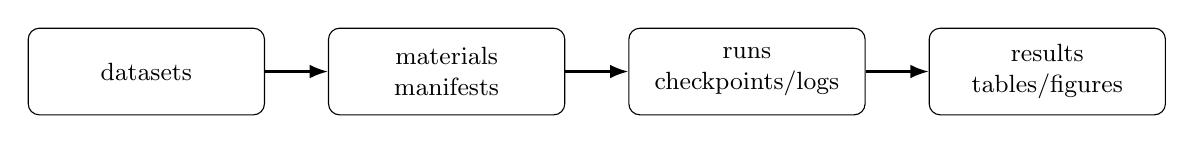
\begin{tikzpicture}[
        font=\small,
        box/.style={draw, rounded corners, align=center, minimum width=3.0cm, minimum height=1.1cm},
        arr/.style={-Latex, thick}
    ]
        \node[box] (data) {datasets};
        \node[box, right=0.8cm of data] (mat) {materials\\manifests};
        \node[box, right=0.8cm of mat] (run) {runs\\checkpoints/logs};
        \node[box, right=0.8cm of run] (res) {results\\tables/figures};
        \draw[arr] (data) -- (mat);
        \draw[arr] (mat) -- (run);
        \draw[arr] (run) -- (res);
    \end{tikzpicture}
    \caption{数据组织与 formal source-of-truth 留档流程}
    \label{fig:formal-working-set-flow}
\end{figure}

\section{本章小结}
本章给出了本文全部正式实验的工作流地基，包括数据来源、val-cal/val-op 划分、统一训练协议以及 manifest-first 的结果留档机制。由此，后续容量扫描、HN sweep 与样本重加权相关实验都可以在同一 formal protocol 下进行比较，而不再依赖零散日志或 trainer 默认输出。

\chapter{高召回门控的 formal 选模与容量扫描}

\noindent 本章要回答三个直接决定后续主线的问题：第一，为什么 stage-1 不能被当作默认阈值二分类处理；第二，在统一 formal protocol 下，哪一个 backbone 才是高召回门控的正式主模型；第三，source six-class 视图与 trainer-side \formalmetric{top1} 为什么都不能替代 direct binary gate 视图。围绕这三个问题，下面依次给出任务重定义、容量扫描主结果、checkpoint 错位证据以及 cross-view mismatch 分析。

\section{stage-1 formal 任务重定义}
\subsection{为什么 stage-1 不是普通二分类}
stage-1 的工程职责不是在默认阈值下获得最高总体分类精度，而是在固定召回约束下尽可能多地拦截 normal，从而降低后续人工复核或后级 detector 的无效负担。因此，若仍以默认阈值 Accuracy 或 trainer-side \formalmetric{top1} 作为主要目标，就会把任务误写成普通二分类，而忽略高召回门控真正关心的 operating point 行为。

\subsection{direct binary gate 作为正式主裁判}
基于这一任务语义，本文将 direct binary gate 明确为 stage-1 的正式主裁判视图。所有 backbone 排序、checkpoint 选择与后续训练侧增强，均必须在 \formalmetric{Spec@R99.5 > Spec@R99.0 > Prec@R99.0 > PTR@R99.0} 这套 formal 排序规则下完成，而不再由 trainer 默认 best 或默认阈值分类得分代替拍板。

\subsection{six-class source 作为辅助参考视图}
与之对应，source-side six-class 视图只承担辅助参考角色。它可以回答 source representation 的容量差异，却不能直接决定 recall-constrained binary gate 的正式 winner。因此，本文在容量扫描章节中始终坚持 ``primary view / auxiliary view'' 的结构安排：binary gate 决定正式主线，six-class 只用于解释 source-side 的容量现象。

\section{direct binary gate formal capacity scan}
\begin{table}[H]
    \centering
    \caption{direct binary gate formal capacity scan 主表}
    \label{tab:stage1-formal-gate-capacity}
    \resizebox{\textwidth}{!}{%
    \begin{tabular}{lcccccccc}
        \toprule
        Model & Best Epoch & Spec@R99.5 & Spec@R99.0 & Prec@R99.0 & PTR@R99.0 & $\tau_{99.5}$ & $\tau_{99.0}$ & Rank \\
        \midrule
        yolo11m-cls & 78  & 0.5952 & 0.6548 & 0.9348 & 0.8829 & 0.2800 & 0.3100 & 1 \\
        yolo11x-cls & 125 & 0.5476 & 0.5952 & 0.9244 & 0.8929 & 0.2900 & 0.3600 & 2 \\
        yolo11l-cls & 54  & 0.5238 & 0.5714 & 0.9205 & 0.8988 & 0.2800 & 0.3000 & 3 \\
        yolo11s-cls & 77  & 0.5238 & 0.5357 & 0.9143 & 0.9028 & 0.2500 & 0.2600 & 4 \\
        yolo11n-cls & 76  & 0.5119 & 0.5833 & 0.9224 & 0.8948 & 0.2500 & 0.3600 & 5 \\
        \bottomrule
    \end{tabular}
    }
\end{table}
\noindent\parbox{\textwidth}{\footnotesize 注：direct binary gate 是 stage-1 的正式选模视图；排序遵循 \formalmetric{Spec@R99.5 > Spec@R99.0 > Prec@R99.0 > PTR@R99.0}。}

\begin{figure}[H]
    \centering
    
\includegraphics[width=0.92\textwidth]{../../../research/results/stage1_formal/capacity_scan/paper_main/figures/fig_stage1_gate_capacity_bar.png}
    \caption{direct binary gate formal capacity scan 的主指标比较}
    \label{fig:stage1-formal-gate-bar}
\end{figure}

表 \ref{tab:stage1-formal-gate-capacity} 表明，在统一的 recall-constrained 排序规则下，\texttt{yolo11m-cls} 在两个主排序锚点 \formalmetric{Spec@R99.5} 与 \formalmetric{Spec@R99.0} 上同时取得最优，并在 \formalmetric{Prec@R99.0} 与 \formalmetric{PTR@R99.0} 上保持最优综合表现。因此，当前 stage-1 formal binary gate 的主模型应固定为 \texttt{yolo11m-cls}，第二对照模型则应固定为 \texttt{yolo11x-cls}。

\section{gate-best checkpoint dynamics}
\begin{figure}[H]
    \centering
    
\includegraphics[width=0.90\textwidth]{../../../research/results/stage1_formal/capacity_scan/paper_main/figures/fig_stage1_gate_spec_r995_curve.png}
    \caption{五模型 \formalmetric{Spec@R99.5} 随 epoch 的演化曲线}
    \label{fig:stage1-formal-gate-spec995}
\end{figure}

\begin{figure}[H]
    \centering
    
\includegraphics[width=0.90\textwidth]{../../../research/results/stage1_formal/capacity_scan/paper_main/figures/fig_stage1_gate_spec_r990_curve.png}
    \caption{五模型 \formalmetric{Spec@R99.0} 随 epoch 的演化曲线}
    \label{fig:stage1-formal-gate-spec990}
\end{figure}

图 \ref{fig:stage1-formal-gate-spec995} 与图 \ref{fig:stage1-formal-gate-spec990} 展示了 formal gate 指标随 checkpoint 变化的整体趋势。五个模型的 gate-best epoch 分别为 \texttt{76/77/78/54/125}（对应 \texttt{n/s/m/l/x}），说明 formal 最优点通常出现在训练中期或后中期，而不是默认意义上的“最后一轮”或“trainer 自动 best”。其中，\texttt{yolo11l-cls} 在较早 epoch 达到峰值，而 \texttt{yolo11x-cls} 需要更长优化轨迹才达到最优，但即便如此，\texttt{yolo11x-cls} 仍未在正式排序下超过 \texttt{yolo11m-cls}。

\section{trainer \formalmetric{top1-best} 与 gate-best 的系统性错位}
\begin{table}[H]
    \centering
    \caption{trainer \formalmetric{top1-best} 与 gate-best 的对照}
    \label{tab:stage1-formal-top1-vs-gatebest}
    \resizebox{\textwidth}{!}{%
    \begin{tabular}{lccccccc}
        \toprule
        Model & Top1-Best Epoch & Top1-Best Top1 & Gate-Best Epoch & Gate-Best Spec@R99.5 & Gate-Best Spec@R99.0 & $\Delta$Epoch & Same \\
        \midrule
        yolo11n-cls & 120 & 0.9250 & 76  & 0.5119 & 0.5833 & 44  & No \\
        yolo11s-cls & 88  & 0.9208 & 77  & 0.5238 & 0.5357 & 11  & No \\
        yolo11m-cls & 197 & 0.9347 & 78  & 0.5952 & 0.6548 & 119 & No \\
        yolo11l-cls & 103 & 0.9306 & 54  & 0.5238 & 0.5714 & 49  & No \\
        yolo11x-cls & 120 & 0.9319 & 125 & 0.5476 & 0.5952 & -5  & No \\
        \bottomrule
    \end{tabular}
    }
\end{table}
\noindent\parbox{\textwidth}{\footnotesize 注：五个模型全部出现 \formalmetric{top1-best} 与 gate-best 不一致；\formalmetric{top1} 可作为训练健康信号，但不应作为 stage-1 的正式早停或检查点选择标准。}

\begin{figure}[H]
    \centering
    
\includegraphics[width=0.92\textwidth]{../../../research/results/stage1_formal/capacity_scan/paper_main/figures/fig_stage1_gate_top1_vs_spec_dualaxis.png}
    \caption{以 \texttt{yolo11m-cls} 与 \texttt{yolo11l-cls} 为例的 \formalmetric{top1} 与 gate 指标错位}
    \label{fig:stage1-formal-gate-top1-mismatch}
\end{figure}

表 \ref{tab:stage1-formal-top1-vs-gatebest} 与图 \ref{fig:stage1-formal-gate-top1-mismatch} 共同揭示了一个关键结论：五个模型中没有任何一个满足 trainer \formalmetric{top1-best} 与 formal gate-best 一致。尤其是 \texttt{yolo11m-cls}，其 trainer 侧 \formalmetric{top1-best} 出现在第 197 轮，而 formal gate-best 出现在第 78 轮，两者相差 119 个 epoch；\texttt{yolo11l-cls} 也表现出类似错位。这一结果说明，trainer 侧的 \formalmetric{top1} 虽然仍能反映分类优化是否正常进行，但并不与 recall-constrained gate objective 对齐。

\section{six-class source formal capacity scan}

\subsection{six-class source 主结果}
\begin{table}[H]
    \centering
    \caption{six-class source formal capacity scan 主表}
    \label{tab:stage1-formal-cls6-capacity}
    \begin{tabular}{lccccc}
        \toprule
        Model & Best Epoch & Accuracy & AUROC & AUPRC & Rank \\
        \midrule
        yolo11x-cls & 161 & 0.7000 & 0.9484 & 0.9885 & 1 \\
        yolo11m-cls & 130 & 0.6958 & 0.9387 & 0.9848 & 2 \\
        yolo11l-cls & 104 & 0.6944 & 0.9400 & 0.9862 & 3 \\
        yolo11s-cls & 167 & 0.6917 & 0.9406 & 0.9854 & 4 \\
        yolo11n-cls & 117 & 0.6833 & 0.9421 & 0.9870 & 5 \\
        \bottomrule
    \end{tabular}
\end{table}
\noindent\parbox{\textwidth}{\footnotesize 注：six-class source 视图仅用于 source-side representation 参考，不承担 stage-1 的正式选模功能。}

\begin{figure}[H]
    \centering
    
\includegraphics[width=0.88\textwidth]{../../../research/results/stage1_formal/capacity_scan/paper_main/figures/fig_stage1_cls6_capacity_bar.png}
    \caption{six-class source formal capacity scan 的五模型比较}
    \label{fig:stage1-formal-cls6-bar}
\end{figure}

在 source-side six-class 任务下，\texttt{yolo11x-cls} 为辅助参考 leader，\texttt{yolo11m-cls} 位居第二。这一结果说明，更大容量模型在源域六类表示任务上仍具有优势；但该优势并不能直接转译为 recall-constrained binary gate 下的正式最优。

\section{cross-view rank mismatch 分析}
\begin{table}[H]
    \centering
    \caption{six-class source 与 direct binary gate 的跨视图排序差异}
    \label{tab:stage1-formal-crossview-rank-gap}
    \resizebox{\textwidth}{!}{%
    \begin{tabular}{lcccc}
        \toprule
        Model & Rank in CLS6 & Rank in Binary Gate & Rank Gap & Interpretation \\
        \midrule
        yolo11x-cls & 1 & 2 & -1 & 辅助 cls6 视图相对高估该模型 \\
        yolo11m-cls & 2 & 1 & 1  & 辅助 cls6 视图相对低估该模型 \\
        yolo11l-cls & 3 & 3 & 0  & 两种视图排序一致 \\
        yolo11s-cls & 4 & 4 & 0  & 两种视图排序一致 \\
        yolo11n-cls & 5 & 5 & 0  & 两种视图排序一致 \\
        \bottomrule
    \end{tabular}
    }
\end{table}

\begin{figure}[H]
    \centering
    
\includegraphics[width=0.88\textwidth]{../../../research/results/stage1_formal/capacity_scan/paper_main/figures/fig_stage1_crossview_rank_gap.png}
    \caption{six-class source 与 direct binary gate 的排序错位可视化}
    \label{fig:stage1-formal-crossview-gap}
\end{figure}

表 \ref{tab:stage1-formal-crossview-rank-gap} 与图 \ref{fig:stage1-formal-crossview-gap} 表明，source six-class 排序不能替代 direct binary gate 排序。最关键的差异集中在 \texttt{yolo11m-cls} 与 \texttt{yolo11x-cls}：前者在 source six-class 中位居第二，却在 binary gate 中成为正式主模型；后者在 source six-class 中位居第一，却在 binary gate 中退居第二。

\section{stage-1 主模型与第二对照模型的确定}
综合 binary gate 主表、checkpoint dynamics、top1-best 与 gate-best 错位表以及 cross-view rank mismatch，可得到一个稳定且不依赖单一辅助视图的结论：\texttt{yolo11m-cls} 是当前 stage-1 formal mainline 的唯一合理主模型，\texttt{yolo11x-cls} 则应作为容量更大的第二对照模型保留。相较之下，\texttt{yolo11l-cls} 虽然在早期 exploratory 阶段具有吸引力，但在当前统一 formal protocol 下已不再承担主线角色。

\section{本章小结}
本章完成了 stage-1 backbone 选择问题的正式闭环。通过把 direct binary gate 与 six-class source 明确区分为 primary view 与 auxiliary view，本文不仅确定了 \texttt{yolo11m-cls} 和 \texttt{yolo11x-cls} 的 mainline 角色，也证明了 trainer-side \formalmetric{top1} 与 source-side capacity 排名都不能替代 formal gate-aware 选模。

\chapter{基于 HN 回流的 stage-1 训练侧增强}

\noindent 本章要回答的问题不是“HN 有没有用”这么宽泛，而是更具体的三件事：其一，在已经固定 backbone mainline 的前提下，HN ratio sweep 是否存在清晰的 sweet spot；其二，这种收益是否是单调的、是否会稳定复现在第二模型上；其三，当前 uniform replay 暗示了哪些尚未解决的样本价值异质性问题。以下结果均沿用与第 4 章一致的 formal evaluator 与正式排序规则。

\section{HN 回流设置与样本来源}
\begin{table}[H]
    \centering
    \caption{\texttt{yolo11m-cls} 的 HN 正式排序主表}
    \label{tab:hn-m-main-ranking}
    \resizebox{\textwidth}{!}{%
    \begin{tabular}{lcccccccccc}
        \toprule
        Ratio & Best Epoch & Spec@R99.5 & Spec@R99.0 & Prec@R99.0 & PTR@R99.0 & Rank & $\Delta$Spec@R99.5 & $\Delta$Spec@R99.0 & $\Delta$Prec@R99.0 & $\Delta$PTR@R99.0 \\
        \midrule
        hn00 & 78  & 0.5952 & 0.6548 & 0.9348 & 0.8829 & 3  & 0.0000  & 0.0000  & 0.0000  & 0.0000 \\
        hn02 & 51  & 0.6429 & 0.6429 & 0.9330 & 0.8889 & 2  & 0.0476  & -0.0119 & -0.0018 & 0.0060 \\
        hn04 & 144 & 0.5595 & 0.6071 & 0.9265 & 0.8909 & 7  & -0.0357 & -0.0476 & -0.0083 & 0.0079 \\
        hn06 & 96  & 0.5952 & 0.6190 & 0.9286 & 0.8889 & 4  & 0.0000  & -0.0357 & -0.0063 & 0.0060 \\
        hn08 & 1   & 0.5833 & 0.6548 & 0.9348 & 0.8829 & 5  & -0.0119 & 0.0000  & 0.0000  & 0.0000 \\
        hn10 & 29  & 0.5238 & 0.5357 & 0.9145 & 0.9048 & 11 & -0.0714 & -0.1190 & -0.0204 & 0.0218 \\
        hn12 & 115 & 0.5357 & 0.5714 & 0.9204 & 0.8968 & 10 & -0.0595 & -0.0833 & -0.0145 & 0.0139 \\
        hn14 & 74  & 0.6429 & 0.6548 & 0.9350 & 0.8849 & 1  & 0.0476  & 0.0000  & 0.0001  & 0.0020 \\
        hn16 & 118 & 0.5714 & 0.5714 & 0.9207 & 0.9008 & 6  & -0.0238 & -0.0833 & -0.0141 & 0.0179 \\
        hn18 & 48  & 0.5476 & 0.5476 & 0.9167 & 0.9048 & 9  & -0.0476 & -0.1071 & -0.0182 & 0.0218 \\
        hn20 & 1   & 0.5595 & 0.5952 & 0.9246 & 0.8948 & 8  & -0.0357 & -0.0595 & -0.0102 & 0.0119 \\
        \bottomrule
    \end{tabular}
    }
\end{table}

\begin{figure}[H]
    \centering
    
\includegraphics[width=0.92\textwidth]{../../../research/results/stage1_formal/gate_hn_paper/figures/fig_hn_m_ratio_metric_curves_panel.png}
    \caption{\texttt{yolo11m-cls} 在不同 HN ratio 下的四项正式指标变化}
    \label{fig:hn-m-ratio-metrics}
\end{figure}

表 \ref{tab:hn-m-main-ranking} 与图 \ref{fig:hn-m-ratio-metrics} 共同表明，HN 的收益不是单调增加，而是存在清晰的 sweet spot。按与 capacity scan 完全一致的 formal 排序规则，\texttt{hn14} 成为 \texttt{yolo11m-cls} 的正式 winner；\texttt{hn02} 虽然在 \formalmetric{Spec@R99.5} 上达到同样的提升幅度，但在 \formalmetric{Spec@R99.0} 与后续 tie-break 上落后于 \texttt{hn14}。

\section{相对 \texttt{hn00} 的增量解释}
\begin{table}[H]
    \centering
    \caption{\texttt{yolo11m-cls} 各 HN ratio 相对 \texttt{hn00} 的紧凑增量表}
    \label{tab:hn-m-delta}
    \resizebox{\textwidth}{!}{%
    \begin{tabular}{lccccc}
        \toprule
        Ratio & Best Epoch & $\Delta$Spec@R99.5 & $\Delta$Spec@R99.0 & $\Delta$Prec@R99.0 & $\Delta$PTR@R99.0 \\
        \midrule
        hn00 & 78  & 0.0000  & 0.0000  & 0.0000  & 0.0000 \\
        hn02 & 51  & 0.0476  & -0.0119 & -0.0018 & 0.0060 \\
        hn04 & 144 & -0.0357 & -0.0476 & -0.0083 & 0.0079 \\
        hn06 & 96  & 0.0000  & -0.0357 & -0.0063 & 0.0060 \\
        hn08 & 1   & -0.0119 & 0.0000  & 0.0000  & 0.0000 \\
        hn10 & 29  & -0.0714 & -0.1190 & -0.0204 & 0.0218 \\
        hn12 & 115 & -0.0595 & -0.0833 & -0.0145 & 0.0139 \\
        hn14 & 74  & 0.0476  & 0.0000  & 0.0001  & 0.0020 \\
        hn16 & 118 & -0.0238 & -0.0833 & -0.0141 & 0.0179 \\
        hn18 & 48  & -0.0476 & -0.1071 & -0.0182 & 0.0218 \\
        hn20 & 1   & -0.0357 & -0.0595 & -0.0102 & 0.0119 \\
        \bottomrule
    \end{tabular}
    }
\end{table}

\begin{figure}[H]
    \centering
    
\includegraphics[width=0.74\textwidth]{../../../research/results/stage1_formal/gate_hn_paper/figures/fig_hn_best_epoch_vs_ratio.png}
    \caption{\texttt{yolo11m-cls} 的 gate-best epoch 随 HN ratio 的变化}
    \label{fig:hn-best-epoch-vs-ratio}
\end{figure}

表 \ref{tab:hn-m-delta} 有助于从 \texttt{hn00} 锚点解释 HN 增益的来源。首先，\texttt{hn14} 的主要贡献来自 \formalmetric{Spec@R99.5} 的显著提升，同时保持 \formalmetric{Spec@R99.0} 基本不变，并在 \formalmetric{Prec@R99.0} 上取得轻微正增益。其次，\formalmetric{PTR@R99.0} 并未同步改善，而是出现 0.0020 的小幅上升，说明当前 formal winner 的收益更集中体现在高召回下的前级 normal filtering，而不是 pass-through rate 的全面下降。图 \ref{fig:hn-best-epoch-vs-ratio} 则表明，gate-best epoch 会随 ratio 发生系统性移动，进一步说明 HN 改变的是训练轨迹，而非仅在终点挑选一个偶然更好的 checkpoint。

\section{代表 ratio 的 epoch dynamics}
\begin{figure}[H]
    \centering
    
\includegraphics[width=0.94\textwidth]{../../../research/results/stage1_formal/gate_hn_paper/figures/fig_hn_m_epoch_dynamics_panel.png}
    \caption{\texttt{hn00}、formal winner 与高比例尾部 ratio 的 epoch dynamics 对比}
    \label{fig:hn-m-epoch-dynamics}
\end{figure}

图 \ref{fig:hn-m-epoch-dynamics} 选取了三种代表性设置：\texttt{hn00}、当前 formal winner \texttt{hn14} 以及高比例尾部设置 \texttt{hn20}。可以看到，HN 不仅影响最终 best checkpoint 的落点，还改变了训练过程中 \formalmetric{Spec@R99.5}、\formalmetric{Spec@R99.0}、\formalmetric{Prec@R99.0} 与 \formalmetric{PTR@R99.0} 的轨迹形态。相较于 \texttt{hn00}，\texttt{hn14} 在 \formalmetric{Spec@R99.5} 上形成更高平台，而 \texttt{hn20} 则显示出更早但更弱的峰值。

\section{与 baseline mainline 的衔接及 cross-capacity validation}
\begin{table}[H]
    \centering
    \caption{baseline mainline 与 HN anchor 的桥接对照}
    \label{tab:hn-bridge}
    \resizebox{\textwidth}{!}{%
    \begin{tabular}{lccccc}
        \toprule
        Setting & Best Epoch & Spec@R99.5 & Spec@R99.0 & Prec@R99.0 & PTR@R99.0 \\
        \midrule
        yolo11m baseline (hn00) & 78  & 0.5952 & 0.6548 & 0.9348 & 0.8829 \\
        yolo11m + hn14          & 74  & 0.6429 & 0.6548 & 0.9350 & 0.8849 \\
        yolo11x baseline (hn00) & 125 & 0.5476 & 0.5952 & 0.9244 & 0.8929 \\
        yolo11x + hn02          & 1   & 0.5238 & 0.5476 & 0.9163 & 0.9008 \\
        \bottomrule
    \end{tabular}
    }
\end{table}

\begin{table}[H]
    \centering
    \caption{\texttt{yolo11x-cls} 的 light HN cross-capacity check}
    \label{tab:hn-x-crosscheck}
    \begin{tabular}{lccccc}
        \toprule
        Ratio & Best Epoch & Spec@R99.5 & Spec@R99.0 & Prec@R99.0 & PTR@R99.0 \\
        \midrule
        hn00 & 125 & 0.5476 & 0.5952 & 0.9244 & 0.8929 \\
        hn02 & 1   & 0.5238 & 0.5476 & 0.9163 & 0.9008 \\
        \bottomrule
    \end{tabular}
\end{table}

\begin{figure}[H]
    \centering
    
\includegraphics[width=0.94\textwidth]{../../../research/results/stage1_formal/gate_hn_paper/figures/fig_hn_cross_capacity_slope_panel.png}
    \caption{\texttt{yolo11m-cls} 与 \texttt{yolo11x-cls} 在 \texttt{hn00} 到 \texttt{hn02} 间的 cross-capacity 方向性对比}
    \label{fig:hn-cross-capacity}
\end{figure}

表 \ref{tab:hn-bridge} 说明，HN 实验与既有 baseline mainline 的衔接方式是“固定 backbone 后做 ratio sweep”，而不是重新开启容量法庭。对于 \texttt{yolo11m-cls}，\texttt{hn14} 相对 \texttt{hn00} 在 \formalmetric{Spec@R99.5} 上取得 0.0476 的绝对提升，并在 \formalmetric{Spec@R99.0} 与 \formalmetric{Prec@R99.0} 上基本保持不变。相比之下，表 \ref{tab:hn-x-crosscheck} 与图 \ref{fig:hn-cross-capacity} 表明，\texttt{yolo11x-cls} 上的 \texttt{hn02} 并未复现相同方向的净增益，四个正式指标均较 \texttt{hn00} 回落。因而，HN 的收益应被理解为与模型容量和训练动力学相关的增强效应，而不是对任意 backbone 都稳定成立的统一规律。

\section{HN 样本来源的可追溯性}
当前 HN working set 还提供了 hard-normal 来源证据。具体而言，\texttt{yolo11m} 的 HN 候选来自 1080 个训练 normal 样本，其中分数最高的 250 个样本构成回流池，占训练 normal 总量的 23.15\%。这意味着本文所讨论的 HN 并非人工主观挑选，而是直接来自 baseline gate 在训练 normal 集上的高风险尾部分布。为控制仓库存储，附录仅保留分布统计与最高分候选名单，而不复制分类图像文件。

\begin{table}[H]
    \centering
    \caption{hard-normal 选样统计}
    \label{tab:hn-hard-normal-stats-main}
    \begin{tabular}{lcccccccc}
        \toprule
        Normal Total & Selected & Ratio & Score Min & Score Median & Score Max & Score P95 & Score P99 & Threshold \\
        \midrule
        1080 & 250 & 0.2315 & 0.1133 & 0.2854 & 0.9780 & 0.8377 & 0.9143 & 0.1133 \\
        \bottomrule
    \end{tabular}
\end{table}

\begin{figure}[H]
    \centering
    
\includegraphics[width=0.92\textwidth]{../../../research/results/stage1_formal/gate_hn_paper/appendix/fig_hn_hard_normal_score_distribution.png}
    \caption{训练 normal 样本的异常分数分布与 hard-normal 选择阈值}
    \label{fig:hn-score-distribution-main}
\end{figure}

\begin{table}[H]
    \centering
    \caption{top-ranked hard-normal candidate list（正文摘录）}
    \label{tab:hn-hard-example-list-main}
    \begin{tabular}{ccccc}
        \toprule
        Rank & Image Name & Image Stub & Predicted Abnormal Score & Heuristic Group \\
        \midrule
        1  & 00467510.png & 00467510 & 0.9780 & 其他 \\
        2  & 00329365.png & 00329365 & 0.9536 & 其他 \\
        3  & 00149587.png & 00149587 & 0.9238 & 其他 \\
        4  & 00130666.png & 00130666 & 0.9043 & 其他 \\
        5  & 00160652.png & 00160652 & 0.8989 & 反光 \\
        6  & 00144495.png & 00144495 & 0.8984 & 反光 \\
        7  & 00323059.png & 00323059 & 0.8921 & 其他 \\
        8  & 00505638.png & 00505638 & 0.8867 & 其他 \\
        9  & 00021678.png & 00021678 & 0.8682 & 其他 \\
        10 & 00022521.png & 00022521 & 0.8545 & 其他 \\
        11 & 00292889.png & 00292889 & 0.8511 & 其他 \\
        12 & 00375607.png & 00375607 & 0.8486 & 反光 \\
        \bottomrule
    \end{tabular}
\end{table}

表 \ref{tab:hn-hard-normal-stats-main}、图 \ref{fig:hn-score-distribution-main} 与表 \ref{tab:hn-hard-example-list-main} 共同说明，当前 hard-normal pool 的来源是训练 normal 高风险尾部，而不是人工主观筛图。选入 top250 pool 的样本最低分数为 0.1133，中位数为 0.2854，最高达到 0.9780；最高分候选中既包含持续高风险的复杂纹理样本，也包含反光等容易诱发高分的视觉模式。考虑到论文仓库不长期保留分类图片副本，正文采用 top-ranked 名单而不是重复拷贝原图缩略图。这一证据已经足以说明 HN 回流面对的是一个内部风险高度不均匀的候选池，也正因此，uniform replay 之后还存在进一步做 fixed-budget 样本重分配的必要性。

\section{HN 回流的已知边界}
尽管 \texttt{yolo11m-cls} 上的 HN sweep 已经证明 uniform hard replay 可以带来正式指标上的可观测净增益，但这一增益具有三条明确边界。第一，收益不是单调随 ratio 增加而增长，而是存在窄 sweet spot。第二，收益不具备 backbone 无关性，\texttt{yolo11x-cls} 的 light validation 已经表明小比例 HN 并不必然复现相同方向的净增益。第三，uniform replay 只能说明 hard pool 作为整体具有训练价值，并不能说明 pool 内部样本价值近似同质；这恰恰构成了后续样本效用重加权方法的直接动机。

\section{本章小结}
本章把 HN 回流从“是否有用”的经验判断推进为“在统一 formal 规则下可排序、可审计、可复核”的训练侧增强问题。当前证据表明，\texttt{yolo11m-cls + hn14} 是主模型上的正式 sweet spot，而 HN 收益同时呈现出非单调、模型相关和候选池内部异质性的特征，这为下一章从比例扫描转向样本价值重分配奠定了经验基础。

\chapter{基于有效信息量的非线性样本重加权方法}

\noindent 本章的任务不是伪造新的已完成性能结论，而是把第 5 章已经暴露出来的问题形式化：当 \texttt{yolo11m-cls + hn14} 已经被确认是 uniform replay 的 sweet spot 后，下一步真正需要回答的就不再是“是否继续扫描比例”，而是“在固定 HN14 预算下，hard-normal pool 内部哪些样本更值得被重复学习”。因此，本章按“现象驱动、理论动机、公式定义、实验设计、结果边界”的顺序组织为一个完整的方法章。

\section{问题提出：从 HN 比例扫描到样本价值建模}
第 5 章已经表明，uniform HN replay 的收益既不是单调的，也不是 backbone 无关的。对于当前主模型 \texttt{yolo11m-cls}，\texttt{hn14} 是固定 formal protocol 下的 sweet spot；但同一方向的收益并未在 \texttt{yolo11x-cls} 上自动复现。由此可见，当前尚未解决的关键变量，已经不再是“HN 要不要加、加多少”，而是“在 fixed-budget 的 hard-normal pool 内，哪些样本更值得被重复学习”。因此，本文将下一步训练侧增强问题形式化为固定预算下的样本价值重分配，而不是重新开启新的 HN ratio sweep。

\section{固定预算样本重分配问题的形式化定义}
设由现有 working set 导出的 hard-normal candidate pool 为
\begin{equation}
\mathcal{N}_{\mathrm{hard}} = \{x_i\}_{i=1}^{250},
\end{equation}
其来源固定为 baseline gate 在训练 normal 集上的 top250 高风险样本。令 uniform \texttt{hn14} 的额外 replay 总预算为 $B$，则本文关注的问题并非扩大候选池或继续增加 HN 数量，而是在总预算固定为 $B$ 的前提下，重新分配 hard pool 内部样本的采样概率：
\begin{equation}
\sum_{i=1}^{250} b_i = B,
\qquad
b_i \propto \pi_i,
\end{equation}
其中 $\pi_i$ 为样本 $x_i$ 的非线性采样概率。当前工作中，$B$ 由既有 \texttt{hn14} working set 决定，因此方法比较的核心不再是“更多回流是否更好”，而是“同样预算下怎样选择更有价值的回流样本”。

\section{Gate-Aligned Effective Information Score 的设计}
为使评分函数与 formal gate objective 对齐，本文首先使用未加回流偏置的 teacher，即 \texttt{yolo11m-cls + hn00} 的 gate-best checkpoint，在 val-cal 上拟合温度参数 $T$，再对 hard-normal pool 中的样本计算校准后 abnormal 概率：
\begin{equation}
p_i = \sigma(z_i / T),
\end{equation}
其中 $z_i$ 为样本 $x_i$ 的 logit 输出，$\sigma(\cdot)$ 为 sigmoid 函数。基于校准后分数，本文构建 lite 版有效信息量评分函数的三个分量。

\subsection{校准后风险项的定义}
首先定义风险项。记当前 teacher 在 \formalmetric{R99.5} 约束下的 operating threshold 为 $\tau_{99.5}$，则风险项定义为
\begin{equation}
r_i = \max\left(0,\frac{p_i-\tau_{99.5}}{1-\tau_{99.5}}\right),
\qquad
R_i = r_i^\alpha,
\end{equation}
其中 $\alpha > 1$ 用于对真正靠近或高于正式门控边界的 normal 施加非线性放大。

\subsection{一致性稳定性项的定义}
其次引入一致性稳定性项。对同一图像施加 $K$ 次轻量、语义保持的 TTA，得到校准后分数 $p_i^{(1)},\dots,p_i^{(K)}$，则其 logit 方差为
\begin{equation}
v_i = \mathrm{Var}\!\left(\operatorname{logit}(p_i^{(1)}),\dots,\operatorname{logit}(p_i^{(K)})\right),
\end{equation}
相应的一致性项定义为
\begin{equation}
C_i = \exp(-v_i/\sigma_c^2),
\end{equation}
其中 $\sigma_c$ 由当前候选池的 robust scale 给出。该项用于抑制“高风险但极不稳定”的样本，避免将 acquisition noise 或伪难例过度放大。

\subsection{结构支撑度项的定义}
第三定义结构支撑度项。对 top250 pool 提取 penultimate features，并在池内计算 $k$ 近邻平均 cosine similarity：
\begin{equation}
d_i = \frac{1}{k}\sum_{j\in kNN(i)} \cos(f_i,f_j),
\qquad
D_i = \mathrm{Norm}(d_i).
\end{equation}
若某个高风险样本在 feature space 中拥有一组结构相近的困难邻居，则它更可能对应可重复出现的系统性混淆模式；反之，孤立异常点则更可能是低可学习价值的噪声样本 \cite{kim2024structural}。

\subsection{最终评分函数与非线性采样概率}
由此，本文定义三种 lite 版评分：
\begin{equation}
S_i^{(A2)} = R_i,
\end{equation}
\begin{equation}
S_i^{(A3)} = (R_i C_i)^{1/2},
\end{equation}
\begin{equation}
S_i^{(A4)} = (R_i C_i D_i)^{1/3}.
\end{equation}
几何平均的目的在于保留“并且成立”的逻辑，即一个样本若想获得高分，必须同时具备靠近正式门控边界、预测稳定以及在 feature space 中具有结构支撑这三个属性。

最后，固定预算采样概率定义为
\begin{equation}
\pi_i = \frac{(S_i+\epsilon)^\kappa}{\sum_j (S_j+\epsilon)^\kappa},
\end{equation}
其中 $\epsilon$ 为数值稳定常数，$\kappa>1$ 控制对高价值样本的非线性放大程度。该设计保证了总预算仍与 uniform \texttt{hn14} 严格等价，只改变 hard pool 内部的 replay 分布，而不改变候选池本身。

\section{Lite 版 5 组消融实验设计}
\begin{table}[H]
    \centering
    \caption{Lite 版 A0--A4 五组实验定义}
    \label{tab:lite-ablation-settings}
    \begin{tabularx}{\textwidth}{p{1.5cm}p{3.6cm}X}
        \toprule
        Setting & 名称 & 定义 \\
        \midrule
        A0 & \texttt{hn00} baseline & 直接复用当前 formal baseline，不进行 HN 回流。 \\
        A1 & \texttt{uniform\_hn14} & 直接复用当前 formal HN winner，对应既有 uniform replay working set。 \\
        A2 & \texttt{weighted\_hn14\_risk\_only} & 固定 top250 hard-normal pool 与 HN14 总预算，只按风险项 $R_i$ 做非线性重加权。 \\
        A3 & \texttt{weighted\_hn14\_risk\_consistency} & 在 A2 基础上加入一致性稳定性项 $C_i$，抑制高风险但极不稳定的样本。 \\
        A4 & \texttt{weighted\_hn14\_risk\_consistency\_density} & 在 A3 基础上再加入结构支撑度项 $D_i$，构成 lite 版最完整设置。 \\
        \bottomrule
    \end{tabularx}
\end{table}

基于上述评分函数，本文将后续实验统一组织为五组 setting。A0 为 \texttt{hn00} baseline，直接复用已完成 formal 结果；A1 为现有 \texttt{uniform\_hn14}，也直接复用正式结果。A2、A3 与 A4 则分别对应 risk-only、risk+consistency 以及 risk+consistency+density 三组新实验，其中 teacher 固定为 \texttt{yolo11m-cls + hn00} 的 gate-best checkpoint，hard pool 固定为现有 top250，额外 replay 总预算固定为 \texttt{hn14} 的 151。换言之，A2--A4 不是新的 backbone 法庭，而是建立在当前 mainline 之上的 fixed-budget sample reallocation study。

\subsection*{A0 / A1：复用 anchor}
A0 与 A1 的作用并不是构成新的实验贡献，而是为后续 weighted replay 提供两个稳定锚点。A0 保留未加 HN 的 \texttt{hn00} baseline，回答“在没有 hard replay 时 formal gate 达到什么水平”；A1 保留已经完成并被证明为当前主模型 sweet spot 的 \texttt{uniform\_hn14}，回答“uniform replay 在相同预算下已经达到什么水平”。后续全部 lite 版重加权结论，都必须相对于这两个锚点解释。

\subsection*{A2：risk-only}
A2 仅使用校准后风险项 $R_i$，目的在于验证一个最直接的问题：如果只把固定预算更集中地压到“更靠近 formal gate 边界”的高风险 normal 上，是否已经足以优于 uniform \texttt{hn14}。这一设置是最轻量的静态重加权基线，同时也是检验“高风险是否等于高价值”的起点。

\subsection*{A3：risk + consistency}
A3 在 A2 的基础上加入一致性项 $C_i$。其核心假设是，真正值得重复学习的 hard negative 不仅风险高，而且应在轻量、语义保持的 TTA 下保持相对稳定。若某个样本对轻微亮度、对比度或 blur 扰动极度敏感，则它更可能是 acquisition noise 或伪难例，而不应在 fixed-budget replay 中被高权重放大。

\subsection*{A4：risk + consistency + density}
A4 进一步加入结构支撑度项 $D_i$，从而把样本评分推进为 “风险 + 稳定性 + 结构支撑” 的三分量几何平均。该设置是 lite 版的完整形式，用于回答 hard-normal pool 中是否存在一类“既高风险、又稳定、且在 feature space 中具有重复出现模式”的高价值样本。

\subsection*{预算对齐与 teacher 设定}
为保持比较合法性，A2--A4 在四个方面均与当前正式主线保持一致：其一，teacher 固定为 \texttt{yolo11m-cls + hn00} 的 gate-best checkpoint，而不是擅自切换到 \texttt{hn14}；其二，hard pool 固定为既有 \texttt{top\_false\_positive\_normals.csv} 对应的 top250，而不是重新从全部 train normal 取新 pool；其三，额外 replay 总预算严格固定为 151，与 \texttt{uniform\_hn14} 完全等价；其四，正式评估仍沿用与第 4、5 章一致的 val-cal、val-op 与 gate-aware ranking protocol。

\begin{table}[H]
    \centering
    \caption{Lite 版主结果表示例（待 full-run 回填）}
    \label{tab:lite-ablation-main-placeholder}
    \resizebox{\textwidth}{!}{%
    \begin{tabular}{lccccccccc}
        \toprule
        Setting & Teacher & Pool & Budget Anchor & Best Epoch & Spec@R99.5 & Spec@R99.0 & Prec@R99.0 & PTR@R99.0 & Formal Rank \\
        \midrule
        A0 & \texttt{hn00} & baseline & -- & 待回填 & 待回填 & 待回填 & 待回填 & 待回填 & 待回填 \\
        A1 & \texttt{uniform\_hn14} & top250 & 151 & 待回填 & 待回填 & 待回填 & 待回填 & 待回填 & 待回填 \\
        A2 & \texttt{hn00 teacher} & top250 & 151 & 待回填 & 待回填 & 待回填 & 待回填 & 待回填 & 待回填 \\
        A3 & \texttt{hn00 teacher} & top250 & 151 & 待回填 & 待回填 & 待回填 & 待回填 & 待回填 & 待回填 \\
        A4 & \texttt{hn00 teacher} & top250 & 151 & 待回填 & 待回填 & 待回填 & 待回填 & 待回填 & 待回填 \\
        \bottomrule
    \end{tabular}
    }
\end{table}

\begin{table}[H]
    \centering
    \caption{Lite 版相对 \texttt{hn00} 的增量表示例（待 full-run 回填）}
    \label{tab:lite-delta-vs-hn00-placeholder}
    \begin{tabular}{lccccc}
        \toprule
        Setting & $\Delta$Best Epoch & $\Delta$Spec@R99.5 & $\Delta$Spec@R99.0 & $\Delta$Prec@R99.0 & $\Delta$PTR@R99.0 \\
        \midrule
        A0 & 0 & 0 & 0 & 0 & 0 \\
        A1 & 待回填 & 待回填 & 待回填 & 待回填 & 待回填 \\
        A2 & 待回填 & 待回填 & 待回填 & 待回填 & 待回填 \\
        A3 & 待回填 & 待回填 & 待回填 & 待回填 & 待回填 \\
        A4 & 待回填 & 待回填 & 待回填 & 待回填 & 待回填 \\
        \bottomrule
    \end{tabular}
\end{table}

\begin{table}[H]
    \centering
    \caption{Lite 版相对 \texttt{uniform\_hn14} 的增量表示例（待 full-run 回填）}
    \label{tab:lite-delta-vs-hn14-placeholder}
    \begin{tabular}{lccccc}
        \toprule
        Setting & $\Delta$Best Epoch & $\Delta$Spec@R99.5 & $\Delta$Spec@R99.0 & $\Delta$Prec@R99.0 & $\Delta$PTR@R99.0 \\
        \midrule
        A1 & 0 & 0 & 0 & 0 & 0 \\
        A2 & 待回填 & 待回填 & 待回填 & 待回填 & 待回填 \\
        A3 & 待回填 & 待回填 & 待回填 & 待回填 & 待回填 \\
        A4 & 待回填 & 待回填 & 待回填 & 待回填 & 待回填 \\
        \bottomrule
    \end{tabular}
\end{table}

\begin{table}[H]
    \centering
    \caption{Lite 版评分分量统计算表示例（待 full-run 回填）}
    \label{tab:lite-score-component-placeholder}
    \begin{tabularx}{\textwidth}{p{1.6cm}p{2.4cm}p{2.0cm}p{1.8cm}p{1.8cm}Xp{1.8cm}}
        \toprule
        Setting & Score Column & Min & Median & Max & Probability Concentration & Top/Bottom IDs \\
        \midrule
        A2 & $R_i$ / $\pi_i$ & 待回填 & 待回填 & 待回填 & 待回填 & 待回填 \\
        A3 & $(R_iC_i)^{1/2}$ / $\pi_i$ & 待回填 & 待回填 & 待回填 & 待回填 & 待回填 \\
        A4 & $(R_iC_iD_i)^{1/3}$ / $\pi_i$ & 待回填 & 待回填 & 待回填 & 待回填 & 待回填 \\
        \bottomrule
    \end{tabularx}
\end{table}

\section{当前实现状态与验证边界}
截至本文定稿时，capacity scan、cross-view mismatch 与 HN ratio sweep 的 formal 结果已经完整落盘，并构成本论文的主要实验依据。基于这些已完成证据，本文进一步完成了 lite 版样本效用重加权的公式定义、脚本组织、preflight 检查与 smoke-test 工作流设计。但 A2--A4 的 full-run 结果尚未纳入当前 completed evidence，因此本章仅报告方法定义、超参数约束和实验设计，不将其作为已完成性能结论写入前文主结果或后文结论条目。这一处理既保证论文主线与真实完成度一致，也为后续把 fixed-budget reweighting 纳入统一的 formal evaluator 提供了清晰接口。

\section{本章小结}
本章的核心作用不是增加新的已完成实验结论，而是在已建立的 stage-1 证据链基础上，把下一步训练侧增强问题从“比例扫描”推进为“固定预算下的样本价值重分配”。由此，stage-1 主线不再局限于 formal backbone selection 与 HN sweet-spot analysis，而进一步具备了向 sample-utility-driven reweighting 演化的明确方法基础。

\chapter{综合讨论与工程启示}

\noindent 本章不再重复前文实验细节，而是回答三个更高层的问题：第一，当前 stage-1 已经建立了哪些可以稳定复述的正式证据；第二，这些证据对未来完整两阶段系统意味着什么；第三，基于现有完成度，本文明确不打算对哪些问题提前下结论。

\section{已建立的 stage-1 正式证据链}
\begin{table}[H]
    \centering
    \caption{stage-1 已建立证据链总表}
    \label{tab:stage1-evidence-chain}
    \begin{tabularx}{\textwidth}{p{3.1cm}p{3.2cm}Xp{2.2cm}}
        \toprule
        证据环节 & 回答的问题 & 当前正式结论 & 状态 \\
        \midrule
        formal capacity scan & 谁是 stage-1 主模型 & \texttt{yolo11m-cls} 为主模型，\texttt{yolo11x-cls} 为第二对照 & 已完成 \\
        top1-vs-gate mismatch & trainer 指标能否直接选模 & 五模型全部 \formalmetric{top1-best != gate-best} & 已完成 \\
        cross-view mismatch & six-class 能否替代 binary gate & source six-class 仅为辅助视图，不能替代 formal gate 选模 & 已完成 \\
        HN ratio sweep & HN 是否存在正式 sweet spot & \texttt{yolo11m-cls + hn14} 为当前 formal winner & 已完成 \\
        info-sampling-lite & fixed-budget reweighting 是否优于 uniform replay & 方法与 preflight 已建立，full-run 结果尚未纳入本文 completed evidence & 进行中 \\
        \bottomrule
    \end{tabularx}
\end{table}

\begin{figure}[H]
    \centering
    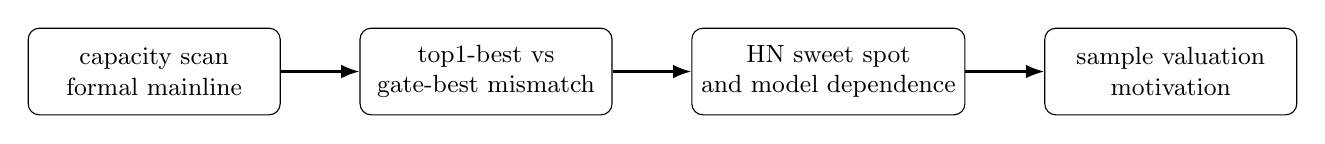
\begin{tikzpicture}[
        font=\small,
        box/.style={draw, rounded corners, align=center, minimum width=3.2cm, minimum height=1.1cm},
        arr/.style={-Latex, thick}
    ]
        \node[box] (cap) {capacity scan\\formal mainline};
        \node[box, right=1.0cm of cap] (mis) {top1-best vs\\gate-best mismatch};
        \node[box, right=1.0cm of mis] (hn) {HN sweet spot\\and model dependence};
        \node[box, right=1.0cm of hn] (lite) {sample valuation\\motivation};
        \draw[arr] (cap) -- (mis);
        \draw[arr] (mis) -- (hn);
        \draw[arr] (hn) -- (lite);
    \end{tikzpicture}
    \caption{从 capacity scan 到 HN 再到有效信息量重加权的逻辑闭环}
    \label{fig:stage1-logic-loop}
\end{figure}

截至当前版本，本文已经建立了四条相互衔接的正式证据链。第一，direct binary gate 是 stage-1 的正式选模视图，而不是默认阈值分类任务的延伸。第二，formal binary gate capacity scan 已经明确给出当前主模型与第二对照模型，即 \texttt{yolo11m-cls} 与 \texttt{yolo11x-cls}。第三，five-model \formalmetric{top1-best} 与 gate-best 的全不一致，证明 trainer-side \formalmetric{top1} 不应再作为 stage-1 的正式选模依据。第四，在主模型已固定的前提下，HN 确实能够在 formal 指标上形成可观测增益，但该增益是非单调、存在 sweet spot 且具有模型相关性的。

\section{对后续两阶段系统的工程启示}
当前结果不支持将 HN 解读为“重新改变全局 backbone 排序”的因素。相反，HN 的合理定位应是：在已完成 capacity scan 的主线上，进一步组织训练样本以提升 recall-constrained filtering 能力。对于 \texttt{yolo11m-cls}，这一增强在 \texttt{hn14} 达到正式最优；对于 \texttt{yolo11x-cls}，当前 light validation 并未提供同方向的净增益。因此，HN 更适合被表述为建立在主模型上的训练侧优化，而不是容量无关的普适策略。

从工程实现角度看，本文对后续两阶段系统至少提供了三点启示。首先，front-end 若要承担减负功能，就必须先 formalize 自身的任务边界、checkpoint 选择和 operating-point 评估方式，否则 stage-2 的输入质量会随 trainer-side proxy 漂移。其次，HN 与未来的样本效用重加权都不应被理解为 detector 替代物，而应被理解为向后级 detector 提供更干净、更稳定前端输入的训练侧机制。最后，即便未来进入 detector 与系统级闭环比较，stage-1 的评价仍应保持独立，因为 source-side classification、default-threshold top1 与 recall-constrained gate objective 并不等价。

\section{本文的局限性与不作出的结论}
\begin{table}[H]
    \centering
    \caption{本文已解决问题与未解决问题对照表}
    \label{tab:stage1-solved-unsolved}
    \begin{tabularx}{\textwidth}{p{4.0cm}Xp{2.4cm}}
        \toprule
        问题类型 & 当前结论 & 是否已闭合 \\
        \midrule
        stage-1 formal 选模 & 已通过 binary gate formal protocol 闭合 & 是 \\
        HN sweet spot & 已在 \texttt{yolo11m-cls} 上闭合到 \texttt{hn14} & 是 \\
        HN 跨容量稳定性 & \texttt{yolo11x-cls} 的 light validation 已提示收益模型相关 & 部分 \\
        fixed-budget 样本重加权效果 & 当前仅完成方法设计、preflight 与 smoke 工作流 & 否 \\
        完整两阶段系统优于单阶段 detector & 当前 manuscript 不作正式结论 & 否 \\
        \bottomrule
    \end{tabularx}
\end{table}

尽管 stage-1 的高召回门控动机来自两阶段系统的工程需求，但当前尚未完成针对单阶段 detector 与两阶段系统的系统级对比实验。因此，本文不对“整体两阶段系统优于单阶段 detector”作出正式结论。当前 manuscript 的有效结论仅限于：若后续系统采用 stage-1 front-end，则其 front-end backbone 与训练侧增强都必须在 direct binary gate 的正式视图下确定，而不能由默认阈值分类指标或 source six-class 结果替代决定。

此外，本文当前尚未报告 Gate-Aligned Effective Information Score lite 的 full-run 结果。第 6 章给出的内容是建立在已完成 stage-1 证据基础上的方法设计与实验框架，而不是新的 completed performance claim。对于 split 尺度、整数步长对阈值定位的影响，以及更大规模跨设备数据条件下的稳定性问题，本文也仅在现有工作流范围内讨论，不对其外推结论作正式声明。

\section{本章小结}
本章的核心作用在于把 capacity scan、HN sweep 与后续样本重加权重新组织为一条闭合的 stage-1 证据链，并明确它对未来两阶段系统研究的意义与边界。换言之，本文已经完成的是 front-end 的 formal 化、选模与训练侧增强，而尚未完成的是 detector 及系统级闭环；这一边界的保留既保证了论证严谨，也为后续工作留出了清晰接口。

\appendix

\chapter{Stage-1 formal protocol 与符号表}
\begin{table}[H]
    \centering
    \caption{Stage-1 formal protocol 摘要}
    \label{tab:stage1-capacity-protocol}
    \begin{tabularx}{\textwidth}{>{\raggedright\arraybackslash}p{3.2cm}X}
        \toprule
        项目 & 说明 \\
        \midrule
        primary selection view & direct binary gate \\
        auxiliary reference view & source six-class capacity scan \\
        binary gate ranking rule & \formalmetric{Spec@R99.5 > Spec@R99.0 > Prec@R99.0 > PTR@R99.0} \\
        six-class ranking rule & Accuracy $>$ AUROC $>$ AUPRC \\
        shared training protocol & \texttt{batch=24}, \texttt{epochs=200}, checkpoint saved every epoch \\
        checkpoint policy & every epoch checkpoint is externally evaluated; trainer \formalmetric{top1} does not determine the official winner \\
        calibration protocol & val-cal temperature fitting followed by val-op threshold sweep \\
        HN protocol & the same calibrated gate-aware rule is reused after backbone selection \\
        manuscript scope & only completed stage-1 evidence is reported in the current paper \\
        \bottomrule
    \end{tabularx}
\end{table}

\chapter{capacity scan 补充材料}

\section{五模型 checkpoint 关键索引}
\begin{table}[H]
    \centering
    \caption{五模型 formal gate-best 与 trainer \formalmetric{top1-best} 关键索引}
    \label{tab:appendix-capacity-checkpoint-index}
    \begin{tabular}{lcccc}
        \toprule
        Model & Gate-Best Epoch & Top1-Best Epoch & Epoch Gap & Binary-Gate Rank \\
        \midrule
        yolo11n-cls & 76  & 120 & 44  & 5 \\
        yolo11s-cls & 77  & 88  & 11  & 4 \\
        yolo11m-cls & 78  & 197 & 119 & 1 \\
        yolo11l-cls & 54  & 103 & 49  & 3 \\
        yolo11x-cls & 125 & 120 & -5  & 2 \\
        \bottomrule
    \end{tabular}
\end{table}

\section{capacity scan 补充说明}
capacity scan 的完整主表、主图与附录图表均已在 \texttt{research/results/stage1\_formal/capacity\_scan/} 下留档。正文只保留最直接支撑结论的主表与主图，而本附录的作用是提供更明确的 checkpoint index、错位量级与 source-of-truth 指向，便于后续复核与复现。

\chapter{HN sweep 与 hard-normal 来源补充材料}

\section{HN 检查点与材料覆盖}
\begin{table}[H]
    \centering
    \caption{HN best checkpoint registry（clean view）}
    \label{tab:hn-registry-clean}
    \resizebox{\textwidth}{!}{%
    \begin{tabular}{lcccccc}
        \toprule
        Model & Ratio & Best Epoch & Spec@R99.5 & Spec@R99.0 & Prec@R99.0 & PTR@R99.0 \\
        \midrule
        yolo11m-cls & hn00 & 78  & 0.5952 & 0.6548 & 0.9348 & 0.8829 \\
        yolo11m-cls & hn02 & 51  & 0.6429 & 0.6429 & 0.9330 & 0.8889 \\
        yolo11m-cls & hn04 & 144 & 0.5595 & 0.6071 & 0.9265 & 0.8909 \\
        yolo11m-cls & hn06 & 96  & 0.5952 & 0.6190 & 0.9286 & 0.8889 \\
        yolo11m-cls & hn08 & 1   & 0.5833 & 0.6548 & 0.9348 & 0.8829 \\
        yolo11m-cls & hn10 & 29  & 0.5238 & 0.5357 & 0.9145 & 0.9048 \\
        yolo11m-cls & hn12 & 115 & 0.5357 & 0.5714 & 0.9204 & 0.8968 \\
        yolo11m-cls & hn14 & 74  & 0.6429 & 0.6548 & 0.9350 & 0.8849 \\
        yolo11m-cls & hn16 & 118 & 0.5714 & 0.5714 & 0.9207 & 0.9008 \\
        yolo11m-cls & hn18 & 48  & 0.5476 & 0.5476 & 0.9167 & 0.9048 \\
        yolo11m-cls & hn20 & 1   & 0.5595 & 0.5952 & 0.9246 & 0.8948 \\
        yolo11x-cls & hn00 & 125 & 0.5476 & 0.5952 & 0.9244 & 0.8929 \\
        yolo11x-cls & hn02 & 1   & 0.5238 & 0.5476 & 0.9163 & 0.9008 \\
        \bottomrule
    \end{tabular}
    }
\end{table}

\begin{table}[H]
    \centering
    \caption{HN ratio 覆盖与材料层级}
    \label{tab:hn-ratio-coverage}
    \resizebox{\textwidth}{!}{%
    \begin{tabular}{lcccccc}
        \toprule
        Model & Ratio & epoch summary & checkpoint index & best manifest & raw per-epoch tree & note \\
        \midrule
        yolo11m-cls & hn00 & Yes & Yes & Yes & No & repo summaries/manifests only; fuller non-PT source archive existed \\
        yolo11m-cls & hn02 & Yes & Yes & Yes & No & repo summaries/manifests only; fuller non-PT source archive existed \\
        yolo11m-cls & hn04 & Yes & Yes & Yes & No & repo summaries/manifests only; fuller non-PT source archive existed \\
        yolo11m-cls & hn06 & Yes & Yes & Yes & No & repo summaries/manifests only; fuller non-PT source archive existed \\
        yolo11m-cls & hn08 & Yes & Yes & Yes & No & repo summaries/manifests only; fuller non-PT source archive existed \\
        yolo11m-cls & hn10 & Yes & Yes & Yes & No & repo summaries/manifests only; fuller non-PT source archive existed \\
        yolo11m-cls & hn12 & Yes & Yes & Yes & No & repo summaries/manifests only; fuller non-PT source archive existed \\
        yolo11m-cls & hn14 & Yes & Yes & Yes & No & repo summaries/manifests only \\
        yolo11m-cls & hn16 & Yes & Yes & Yes & No & repo summaries/manifests only \\
        yolo11m-cls & hn18 & Yes & Yes & Yes & No & repo summaries/manifests only \\
        yolo11m-cls & hn20 & Yes & Yes & Yes & No & repo summaries/manifests only \\
        yolo11x-cls & hn00 & Yes & Yes & Yes & No & repo summaries/manifests only \\
        yolo11x-cls & hn02 & Yes & Yes & Yes & No & repo summaries/manifests only \\
        \bottomrule
    \end{tabular}
    }
\end{table}

\section{HN sweep 的整体形态}
\begin{figure}[H]
    \centering
    
\includegraphics[width=0.88\textwidth]{../../../research/results/stage1_formal/gate_hn_paper/appendix/fig_hn_overview_heatmap_delta.png}
    \caption{各 HN ratio 相对 \texttt{hn00} 的增量热力图}
    \label{fig:hn-heatmap-delta}
\end{figure}

\section{HN 样本来源证明}
\begin{table}[H]
    \centering
    \caption{hard-normal 选样统计}
    \label{tab:hn-hard-normal-stats}
    \begin{tabular}{lcccccc}
        \toprule
        Total Normals & Selected & Ratio & Score Min & Score Median & Score Max & Threshold \\
        \midrule
        1080 & 250 & 0.2315 & 0.1133 & 0.2854 & 0.9780 & 0.1133 \\
        \bottomrule
    \end{tabular}
\end{table}

\begin{figure}[H]
    \centering
    
\includegraphics[width=0.92\textwidth]{../../../research/results/stage1_formal/gate_hn_paper/appendix/fig_hn_hard_normal_score_distribution.png}
    \caption{训练 normal 样本的异常分数分布与 hard-normal 选择阈值}
    \label{fig:hn-score-distribution}
\end{figure}

\begin{table}[H]
    \centering
    \caption{top-ranked hard-normal candidate list}
    \label{tab:hn-hard-example-list}
    \begin{tabular}{ccccc}
        \toprule
        Rank & Image Name & Image Stub & Predicted Abnormal Score & Heuristic Group \\
        \midrule
        1  & 00467510.png & 00467510 & 0.9780 & 其他 \\
        2  & 00329365.png & 00329365 & 0.9536 & 其他 \\
        3  & 00149587.png & 00149587 & 0.9238 & 其他 \\
        4  & 00130666.png & 00130666 & 0.9043 & 其他 \\
        5  & 00160652.png & 00160652 & 0.8989 & 反光 \\
        6  & 00144495.png & 00144495 & 0.8984 & 反光 \\
        7  & 00323059.png & 00323059 & 0.8921 & 其他 \\
        8  & 00505638.png & 00505638 & 0.8867 & 其他 \\
        9  & 00021678.png & 00021678 & 0.8682 & 其他 \\
        10 & 00022521.png & 00022521 & 0.8545 & 其他 \\
        11 & 00292889.png & 00292889 & 0.8511 & 其他 \\
        12 & 00375607.png & 00375607 & 0.8486 & 反光 \\
        \bottomrule
    \end{tabular}
\end{table}

\section{关于 ratio 级 top1-vs-gatebest 的说明}
当前 HN material level 并不包含可靠的 trainer-side per-ratio \formalmetric{top1} 轨迹字段；因此，本文不构造伪造性的 “ratio-level top1-vs-gatebest” 结论，而仅在附录 source-of-truth 中登记该限制。

\chapter{有效信息量评分函数、消融接口与样本清单}

\section{Lite 版评分函数摘要}
为便于后续复现实验，本文将 Gate-Aligned Effective Information Score lite 的最终表达统一记为
\begin{equation}
S_i^{(A2)} = R_i,\qquad
S_i^{(A3)} = (R_i C_i)^{1/2},\qquad
S_i^{(A4)} = (R_i C_i D_i)^{1/3},
\end{equation}
其中风险项 $R_i$、一致性项 $C_i$ 与结构支撑项 $D_i$ 的定义见第 6 章。三组实验共享同一 hard-normal candidate pool、同一 \texttt{hn14} 预算锚点以及同一 formal evaluator，不改变 backbone、batch、epochs 或 checkpoint policy。

\section{样本清单与固定预算接口}
对于 lite 版重加权实验，本文保留的最小可复现 working set 包括候选池 score 清单、采样概率清单、weighted replay 清单与 suite-level summary，而不要求在论文仓库内长期保留全量中间张量或分类图片副本。更具体地说，\texttt{candidate\_pool\_scores.csv}、\texttt{score\_stats.json/md}、\texttt{weighted\_replay\_summary.json} 以及相应 manifest 共同构成了从 fixed top250 pool 到固定预算 replay 分配的可追溯接口。

\chapter{复现实验命令、目录结构与 source-of-truth 清单}

\section{训练脚本与运行入口}
当前 lite 版重加权实验的训练入口统一为 \texttt{main.py} 中的 \texttt{stage1\_formal\_gate\_info\_sampling\_lite} 任务。其脚本组织如下：
\begin{enumerate}[label=\arabic*.]
    \item \texttt{stage1\_prepare\_info\_sampling\_lite\_scores.py}：生成 top250 pool 的 one-shot score、采样概率与 score statistics；
    \item \texttt{stage1\_build\_info\_sampling\_lite\_dataset.py}：在固定 \texttt{hn14} 预算下构建 weighted replay 数据集视图；
    \item \texttt{stage1\_formal\_gate\_info\_sampling\_lite.py}：组织 preflight、smoke、full-run 和 suite-level summary；
    \item \texttt{stage1\_build\_info\_sampling\_lite\_paper\_assets.py}：生成 tables、figures、summary 与 manifests。
\end{enumerate}
为避免误用，teacher 固定为 \texttt{yolo11m-cls + hn00} 的 gate-best checkpoint，hard pool 固定为既有 \texttt{top\_false\_positive\_normals.csv}，budget 固定为 151。若 preflight 或 smoke 未通过，本文不建议直接启动 full-run。

\section{目录结构与 source-of-truth 清单}
与 lite 版实验直接相关的正式目录可概括为三层：其一，\texttt{research/materials/stage1\_formal/gate\_info\_sampling\_lite} 用于保留候选池打分、dataset manifest 与 run manifest；其二，\texttt{research/results/stage1\_formal/gate\_info\_sampling\_lite} 用于保留 PREFLIGHT、SMOKE、SUMMARY、REPRODUCE 与 ARTIFACTS 等汇总文件；其三，\texttt{YOLOv11/datasets/stage1\_formal\_gate\_info\_sampling\_lite} 与 \texttt{YOLOv11/runs/stage1\_formal\_gate\_info\_sampling\_lite} 则分别保存 weighted dataset view 和训练运行目录。三层目录之间通过 manifest 与 path pointer 关联，而不依赖人工整理。

\section{artifacts 保留与清理规则}
考虑到训练侧工作流会产生大量中间文件，本文对 lite 版 artifacts 的保留规则作如下约定：保留 \texttt{candidate\_pool\_scores.csv}、\texttt{score\_stats.json/md}、\texttt{dataset\_manifest.json}、\texttt{run\_manifest.json}、\texttt{epoch\_gate\_summary.*}、\texttt{best\_epoch\_manifest.json} 与 suite-level 主表主图；不将全量 checkpoint 复制到 \texttt{research/materials}，也不默认复制分类图片副本。若临时生成 feature tensor、TTA raw array 或 gallery 中间件，应用后即清理，并在相应 manifest 中登记“已清理”状态。

\backmatter
\begin{thebibliography}{99}
\bibitem{moradi2019review}
Moradi S, Zayed T, Golkhoo F. Review on Computer Aided Sewer Pipeline Defect Detection and Condition Assessment[J]. Infrastructures, 2019, 4(1): 10.

\bibitem{haurum2020survey}
Haurum J B, Moeslund T B. A Survey on Image-Based Automation of CCTV and SSET Sewer Inspections[J]. Automation in Construction, 2020, 111: 103061.

\bibitem{ma2026stateoftheart}
Ma D, Fang H, Wang N, et al. The State-of-the-Art in Pipe Defect Inspection with Computer Vision-Based Methods[J]. Measurement, 2026, 257: 118431.

\bibitem{halfawy2014hogsvm}
Halfawy M R, Hengmeechai J. Automated Defect Detection in Sewer Closed Circuit Television Images Using Histograms of Oriented Gradients and Support Vector Machine[J]. Automation in Construction, 2014, 38: 1--13.

\bibitem{kumar2018cnn}
Kumar S S, Abraham D M, Jahanshahi M R, et al. Automated Defect Classification in Sewer Closed Circuit Television Inspections Using Deep Convolutional Neural Networks[J]. Automation in Construction, 2018, 91: 273--283.

\bibitem{cheng2018deep}
Cheng J C P, Wang M. Automated Detection of Sewer Pipe Defects in CCTV Images Using Deep Learning Techniques[J]. Automation in Construction, 2018, 95: 155--171.

\bibitem{haurum2021sewerml}
Haurum J B, Moeslund T B. Sewer-ML: A Multi-Label Sewer Defect Classification Dataset and Benchmark[C]//Proceedings of the IEEE/CVF Conference on Computer Vision and Pattern Recognition. 2021: 13456--13467.

\bibitem{redmon2016yolo}
Redmon J, Divvala S, Girshick R, Farhadi A. You Only Look Once: Unified, Real-Time Object Detection[C]//Proceedings of the IEEE Conference on Computer Vision and Pattern Recognition. 2016: 779--788.

\bibitem{guo2017calibration}
Guo C, Pleiss G, Sun Y, Weinberger K Q. On Calibration of Modern Neural Networks[C]//Proceedings of the 34th International Conference on Machine Learning. 2017: 1321--1330.

\bibitem{kumar2021constrained}
Kumar A, Narasimhan H, Cotter A, Gupta M. Optimizing Specificity at a High Sensitivity[C]//Proceedings of the 38th International Conference on Machine Learning. 2021: 11415--11424.

\bibitem{koh2017influence}
Koh P W, Liang P. Understanding Black-box Predictions via Influence Functions[C]//Proceedings of the 34th International Conference on Machine Learning. 2017: 1885--1894.

\bibitem{ash2020badge}
Ash J T, Zhang C, Krishnamurthy A, Langford J, Agarwal A. Deep Batch Active Learning by Diverse, Uncertain Gradient Lower Bounds[C]//International Conference on Learning Representations. 2020.

\bibitem{wu2022entropy}
Wu J, Zhang T, Zhai Y, et al. Entropy-Based Active Learning for Object Detection With Progressive Diversity Constraint[C]//Proceedings of the IEEE/CVF Conference on Computer Vision and Pattern Recognition. 2022: 9397--9406.

\bibitem{yang2024plug}
Yang Y, Wu Z, Wang J, et al. Plug-and-Play Active Learning for Object Detection[C]//Proceedings of the IEEE/CVF Conference on Computer Vision and Pattern Recognition. 2024: 25163--25172.

\bibitem{kim2024structural}
Kim M, Hwang J, Kim S, et al. Learning With Structural Labels for Learning With Noisy Labels[C]//Proceedings of the IEEE/CVF Conference on Computer Vision and Pattern Recognition. 2024: 17639--17649.

\bibitem{zhang2024tdds}
Zhang Y, Li X, Zhou Y, et al. Spanning Training Progress: Temporal Dual-Depth Scoring (TDDS) for Enhanced Dataset Pruning in Object Detection[C]//Proceedings of the IEEE/CVF Conference on Computer Vision and Pattern Recognition. 2024: 17665--17675.

\bibitem{situ2023transfer}
Situ Z, Teng S, Feng W, et al. A Transfer Learning-Based YOLO Network for Sewer Defect Detection in Comparison to Classic Object Detection Methods[J]. Developments in the Built Environment, 2023, 15: 100191.

\bibitem{wang2023improvedyolov5}
Wang T, Li Y, Zhai Y, et al. A Sewer Pipeline Defect Detection Method Based on Improved YOLOv5[J]. Processes, 2023, 11(8): 2508.

\bibitem{zhao2024yolov5sewer}
Zhao X, Xiao N, Cai Z, et al. YOLOv5-Sewer: Lightweight Sewer Defect Detection Model[J]. Applied Sciences, 2024, 14(5): 1869.
\end{thebibliography}

\end{document}
